% !TeX root = ../thuthesis-example.tex

\chapter{关键技术}

简述云原生技术背景,云原生应用开发范式,Kubernetes作为云原生的事实标准……
TBD


\section{容器化机器学习}

容器化技术在机器学习平台中的应用具有深远的意义,为模型开发、训练、部署以及维护的全生命周期带来了革命性的变革。
通过将机器学习任务封装在轻量级、可移植的容器中,平台实现了环境的一致性、高效的资源利用以及敏捷的开发流程。

首先,容器化显著提升了环境的一致性和可移植性。
传统的机器学习开发常因不同硬件配置、依赖库版本或操作系统环境的差异而导致代码难以复现或迁移。
而容器技术通过将代码、依赖项和运行时环境打包为独立的镜像,确保了任务在开发、测试和生产环境中的行为一致。
这种一致性不仅减少了环境调试的时间,也大幅降低了模型部署过程中因环境差异导致的失败风险,使得开发者能够专注于模型优化。

其次,容器化提高了资源利用率和任务隔离能力。
在共享资源的机器学习平台中,不同任务之间的资源竞争可能导致性能下降或干扰。
而容器通过轻量级的虚拟化机制,为每个任务提供隔离的运行环境,确保资源分配的独立性和公平性。
同时,容器的快速启动特性能够显著降低资源调度的开销,支持大规模并发任务的高效执行。
此外,容器化结合资源调度器(如Kubernetes)能够对计算资源进行精细化的管理,按需分配CPU、GPU和内存,从而最大化平台的资源利用率。

容器化还大幅提升了开发和部署的效率。
通过定义标准化的容器镜像,开发者可以快速构建和共享模型运行环境,而无需手动配置复杂的依赖项。
此外,容器技术支持持续集成和持续部署(CI/CD)流程,使得模型从开发到上线的过程更加自动化和敏捷。
这种高效的工作流不仅缩短了开发周期,也为快速迭代和试验提供了可能性,尤其在需要频繁更新和调整模型的场景中表现尤为突出。

在分布式训练任务中,容器化技术的价值尤为明显。
现代机器学习模型往往需要通过多节点协同训练来处理海量数据和参数,而容器化可以确保每个节点上的环境一致,避免因环境不一致导致的训练中断。
同时,结合容器编排工具,平台可以自动化地完成训练节点的扩展和故障恢复,显著提高分布式训练的稳定性和效率。

此外,容器化为机器学习任务的监控和运维提供了便利。
容器内任务的日志、性能指标和运行状态可以通过标准化的工具实时采集和分析,便于平台管理员快速定位和解决问题。
与传统运行方式相比,容器化的这种透明性大幅提升了机器学习平台的可维护性。

在生产环境中,容器化的另一个重要价值是支持跨平台和多云部署。
由于容器技术的高度可移植性,机器学习任务可以轻松在本地数据中心、公有云和边缘计算设备之间迁移,而无需担心底层硬件或平台的差异。
这种灵活性不仅为企业节约了运维成本,也使得平台具备了更高的弹性,能够应对不同场景和业务需求。


\section{计算资源池化}

计算资源池化是现代机器学习平台的重要基础架构之一,通过将分散的计算资源整合为统一的资源池,极大地提升了资源利用效率、计算灵活性和平台的可扩展性,其意义和价值在多个方面尤为突出。

首先,计算资源池化能够显著提升资源的利用率。
在传统的固定资源分配模式中,不同任务间的资源往往相互隔离,导致计算能力被闲置或无法动态调整。
而通过池化,所有计算节点的CPU、GPU、NPU等资源可以被集中管理,平台可以根据实际任务需求动态调度资源,从而避免资源浪费。
同时,计算资源池化通过按需分配的方式,支持高并发的任务执行,有效应对多用户、多任务的复杂应用场景。

其次,池化的计算资源提供了极大的灵活性和可扩展性。机器学习任务的需求差异很大,可能包括小规模的实验性模型训练,也可能涉及大规模分布式训练。
计算资源池化使平台能够灵活响应这些需求变化,无需重新配置硬件。
特别是在分布式训练中,池化资源可以支持动态扩展训练节点的数量,满足模型从实验阶段到大规模部署过程中的逐步扩展需要。
此外,当任务结束时,资源会自动释放并返回池中,以便为后续任务重新分配。

计算资源池化还有效促进了多种异构计算资源的协同工作。
在现代机器学习任务中,传统的CPU计算已经无法满足深度学习模型对高性能计算的需求,而GPU、NPU等专用加速硬件成为主力。
通过池化,将这些异构资源统一整合在一起,平台可以为不同任务选择最合适的计算资源。
例如,高并发的推理任务可以优先使用NPU,而复杂的深度学习训练任务则可以分配多卡GPU集群,从而最大化各类硬件的性能潜力。

与此同时,计算资源池化对资源调度和隔离提供了强有力的支持。
在共享环境中,多个用户和任务需要同时使用计算资源。
池化通过精细化的资源分配和调度策略,确保资源分配的公平性和任务执行的效率。
此外,资源池化通过容器化或虚拟化技术,可以在逻辑上隔离不同任务,避免资源竞争和相互干扰,保障每个任务的稳定运行。

另一个显著价值在于成本优化。
计算资源池化能够最大程度地降低硬件成本,通过集中式管理和自动化调度减少过度采购的需求。
同时,在云计算环境中,池化资源与弹性伸缩机制结合,使得平台可以根据负载动态调整资源规模,从而优化成本支出。
此外,通过整合异构计算资源和共享使用,企业可以减少为每种计算需求单独采购专用硬件的必要性。

在实际应用中,计算资源池化直接推动了机器学习平台的生产效率。
它不仅提升了任务的执行效率和资源利用率,还显著缩短了模型开发与训练的周期。
更重要的是,池化架构为机器学习平台提供了更高的弹性和适应性,能够快速响应业务需求的变化,满足从科研实验到大规模生产环境的各种需求。


\section{分布式存储}

分布式存储系统在现代机器学习平台中具有重要的意义,其价值体现在数据管理、性能优化、弹性扩展、高可靠性以及与机器学习框架的深度集成等多个方面。

首先,分布式存储系统在处理海量数据方面展现出卓越的能力。
随着机器学习任务所需数据量的不断增加,从TB到PB级别的规模成为常态,分布式存储通过数据的分片和分散存储,提供了横向扩展的能力,使得存储容量和性能能够随着业务需求的增长而动态调整。
此外,其支持结构化、半结构化和非结构化数据的存储,能够适应机器学习场景中多样化的数据类型需求,如图像、文本和视频等,为模型的开发和训练提供了灵活性。

在性能方面,分布式存储通过并行数据访问机制,显著提升了数据读取和写入的效率。
这对于训练大规模机器学习模型尤为重要,因为高吞吐量和低延迟的数据访问可以有效缩短训练时间。
同时,分布式存储系统通过数据局部性优化,将数据放置在靠近计算节点的位置,从而减少数据传输延迟,提高训练效率。
这种设计尤其适用于分布式训练环境,可以充分利用计算和存储资源。

分布式存储的弹性扩展能力也是其核心优势之一。
与传统存储系统不同,它能够根据实际需求动态增加或减少存储节点,不受物理资源限制,尤其适合机器学习平台从实验室阶段到大规模生产环境的快速扩展需求。
与此同时,通过资源共享与隔离机制,分布式存储在多租户环境下可以实现高效的资源利用,并通过细粒度的权限管理确保数据的安全性。

在可靠性方面,分布式存储通过多副本机制和分布式一致性协议,实现了高容错能力,能够在硬件故障或节点失效的情况下快速恢复数据,确保机器学习任务的连续性。
它还支持快照和备份功能,使模型训练的中间状态能够随时保存与回滚,为迭代开发和实验提供了极大的便利。

此外,分布式存储系统与主流机器学习框架之间的深度集成也是其价值的重要体现。
现代框架如TensorFlow、PyTorch和MindSpore能够直接接入分布式存储系统,统一的数据访问接口简化了开发流程。
同时,通过与数据预处理管道协作,分布式存储能够支持分布式数据加载和分片,加速训练数据准备阶段,为大规模分布式训练任务提供坚实的基础。

从成本和资源利用角度看,分布式存储通过软件定义存储技术,充分利用标准化硬件资源,降低了存储系统的总体拥有成本。
同时,分层存储机制将高频访问的数据存储在高性能设备上,而低频访问的数据则存储在廉价存储介质上,进一步优化了性能与成本的平衡。


\section{分布式训练引擎}

人工智能是如今计算机领域发展迅猛的一个方向,尤其是大模型的横空出世及其应用展现出的强大能力,给未来带来了无限的想象空间。

在大模型大放异彩的背后,大模型的训练是一个复杂的大规模系统工程,涵盖了机器学习理论、计算机系统结构、分布式计算和软件工程等多个计算机科学研究领域。
大模型的训练可以视为大规模的分布式训练,往往需要用到几十到上千台机器(后文的机器指的是带有GPU的AI服务器)协同工作数十天。
本节着重介绍云原生场景下分布式训练的相关技术。

\subsection{背景问题}
如今,许多相关工作者正在致力于优化和加速大模型的训练过程,大模型训练涉及的技术栈较多,主要可以划分为以下三个层次:硬件层、框架层和平台层。
其中,AI平台能够提供数据处理、模型训练、模型推理等服务,管理和调度整个集群的资源,与底层机器交互并进行集群运维,使得用户不需要关心机器硬件方面的问题,能够专注于算法层面上的研究。
因此,平台的功能是否完善、是否能帮助算法工程师减少不必要的时间浪费,对提升模型训练效率至关重要。

由于AI平台会面向很多用户,并且肩负着大规模分布式机器资源管理的职责,因此,AI平台通常会和适用于大规模优化的“云计算”技术紧密关联。
同时,随着云计算的发展逐渐成熟,业界出现了云原生分布式训练的相关技术。
云原生充分利用了云计算提供的基础资源和弹性伸缩的能力,能够构建迭代速度更快、资源利用率更高、容错能力更强的应用程序。
分布式训练是AI平台必须具备的功能,换言之,AI平台需要支持大参数量模型的训练。
此外,当前市场上的算力是十分昂贵的。
例如,一张NVIDIA A100每月的租赁价格大约16000元。
在大规模的分布式训练过程中有机器发生故障的频率会随着机器数量的增长而大幅度增加。
因此分布式训练会经常出现因为机器故障导致训练任务失败的情况,不仅会导致训练开发效率降低,而且会导致大量的时间与金钱的浪费。
为解决上述问题,AI平台具有为分布式训练提供运行保障的能力也非常关键,例如自动重启失败的训练、自动检测GPU是否存在故障、提供方便调试的途径等。

\subsection{分布式训练技术}
分布式训练是一种通过多个分布式的AI服务器计算节点协同工作以加速机器学习模型训练过程的技术。
分布式训练能够有效利用并行计算的优势,通过将大型计算任务分解成若干子任务,并将这些子任务分配到多台机器上执行,从而缩短训练时间,提升训练效率。
下面将从分布式训练的并行策略、通信操作以及目前主流机器学习框架开展研究分析。

分布式训练的核心问题是:数据和模型如何分配到不同的计算节点上,各个节点上的计算结果又如何汇总,才能更有效地缩短训练时间,提升训练效率。
针对该问题,国内外研究学者分别在并行策略和通信操作两方面做了大量研究工作。
当前分布式训练的并行策略主要研究并行计算的模式,目前常见的并行策略主要有以下几类:

(1)数据并行(Data Parallelism)思想早在并行计算兴起初期就已出现,在机器学习兴起之后,也自然而然地移植到了分布式训练之中。
具体方法是将大数据集分割成多个小数据批次,每个计算节点独立处理一个批次的数据,并在所有节点上共享模型参数,各个节点通过梯度平均化或类似的方法同步模型更新。

(2)模型并行(Model Parallelism)是将大型模型划分为多个部分,每个计算节点负责模型的一部分。
节点之间通过特定的通信机制交换中间结果,共同更新整个模型的参数。其中,Megatron就主要参考了模型并行的思想。

(3)流水线并行(Pipeline Parallelism)是模型并行的改进版本,将模型的训练过程按层或阶段划分,形成一个流水线式的处理流程,每个节点专注于模型的一部分并在节点间传递中间结果。
目前有在机器学习框架中实现流水线并行的工作,如GPipe。

(4)参数服务器架构(Parameter Server)是将集群的一个或多个节点作为中心化的参数服务器,用于存储和管理模型参数,其他节点则负责计算并上传梯度,参数服务器接收到梯度后更新模型参数,然后再分发给参与训练的其他节点。
这一架构的缺点在于参数服务器的数据传输量非常巨大,因此现在已经较少使用。

(5)混合并行策略则是结合了数据并行、模型并行和其他技术,以适应更加复杂的训练场景和资源分配需求。
特别是在大模型的训练中,开发者通常不会单一地使用某种并行计算模式,而是手动设计并行方式。
图\ref{fig:disttraining}展示了一种同时采取了模型并行和数据并行的分布式并行策略,将 256 张 GPU 分成 32 组,每组内的 8 张GPU做模型并行,同时 32 组之间进行数据并行,从而实现数百张GPU的分布式训练。

\begin{figure}
  \centering
  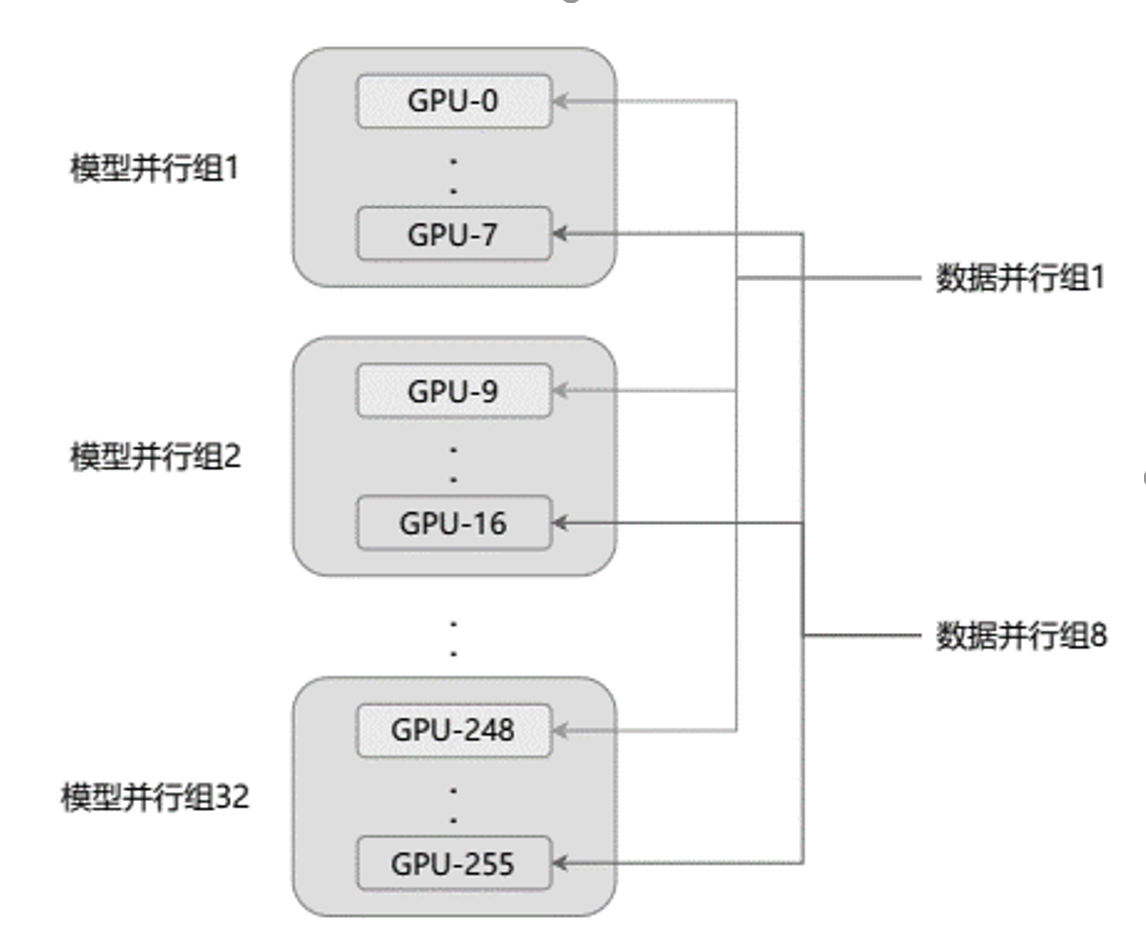
\includegraphics[width=0.6\linewidth]{dist-training.png}
  \caption{分布式训练混合并行策略示意}
  \label{fig:disttraining}
\end{figure}

分布式训练中会涉及节点之间的通信操作,通信操作指的是在多个计算节点之间交换信息,以确保模型训练过程中的数据一致性、梯度同步和参数更新的过程。
常见的分布式通信操作如下:

(1)Scatter(散播)操作是指将一个大的数据集或模型参数分割成多个部分,并将这些部分均匀地分配到不同的计算节点上,每个节点独立处理自己分得的那一部分数据或参数。

(2)Reduce(归约)操作是将分布在多个节点上的相同类型的数据通过某种操作聚合到一起,得到一个全局的结果。
例如,在深度学习训练过程中,各个节点各自计算出局部梯度后, Reduce 操作会将所有节点上的梯度累加起来,得出整个模型的全局梯度。

(3)AllReduce 操作整合了 Scatter 和 Reduce 操作,并将归约后的结果同步到所有参与计算的节点上。
在分布式训练中, AllReduce 对数据并行的训练十分重要,能够确保所有节点在一轮迭代结束后拥有相同的模型参数更新值。

(4)Ring AllReduce是AllReduce的优化版本,其特点是利用环形网络拓扑来进行数据交换和归约操作。
在 Ring AllReduce中,每个节点仅与其相邻的两个节点进行通信,形成一个环状结构。
整个过程分为若干轮次,每一轮中每个节点向其右侧节点发送一半数据,并从左侧节点接收另一半数据,同时在接收过程中对收到的数据与本地数据进行相应的运算。
通过这种方式,所有节点逐步累积并更新数据,直到所有节点都获得了完整的全局运算结果。
Ring AllReduce的通信成本复杂度较低,在大规模GPU集群中特别受欢迎,大大提高了分布式训练的效率和可扩展性。

\subsection{主流机器学习框架}

机器学习框架是指一种专门设计的软件开发工具包或平台,为开发者提供了标准化的接口、模块化组件和预先实现的算法集合,以支持机器学习模型的快速开发、训练、验证、优化以及部署。
常见的机器学习框架有PyTorch、TensorFlow、MXnet、Caffe、Xgboost等,其中PyTorch是目前使用人数最多的机器学习框架,框架中对分布式训练也有支持。

\subsection{云原生分布式训练}

云原生是一种构建和运行应用程序的方法论,充分利用了云计算的弹性和可扩展性,结合现代化的软件开发实践,确保应用程序能够在公有云、私有云和混合云环境中无缝运行和高效管理。
云原生包含的关键技术有容器技术、容器编排系统、微服务治理工具、DevOps工具链等。

Kubernetes是目前最流行的实现云原生理念的容器编排系统,是开发云原生应用的关键基础设施。
从功能角度出发,Kubernetes系统可以大致分为管控和资源两大部分:管控部分涉及Kubernetes系统的管理和资源的控制功能,通常由系统中持续运行的组件完成。
资源主要指系统中被管理和调度的对象,有更新较频繁、具有动态性质的资源(如Pod),也有在系统中长期存在、相对静态的资源(如自定义资源CRD)。
在实际实现分布式训练时,需要用到一些别的组件和资源。
分布式涉及到相关组件和资源的架构如图\ref{fig:disttrainingk8s}所示。

\begin{figure}
  \centering
  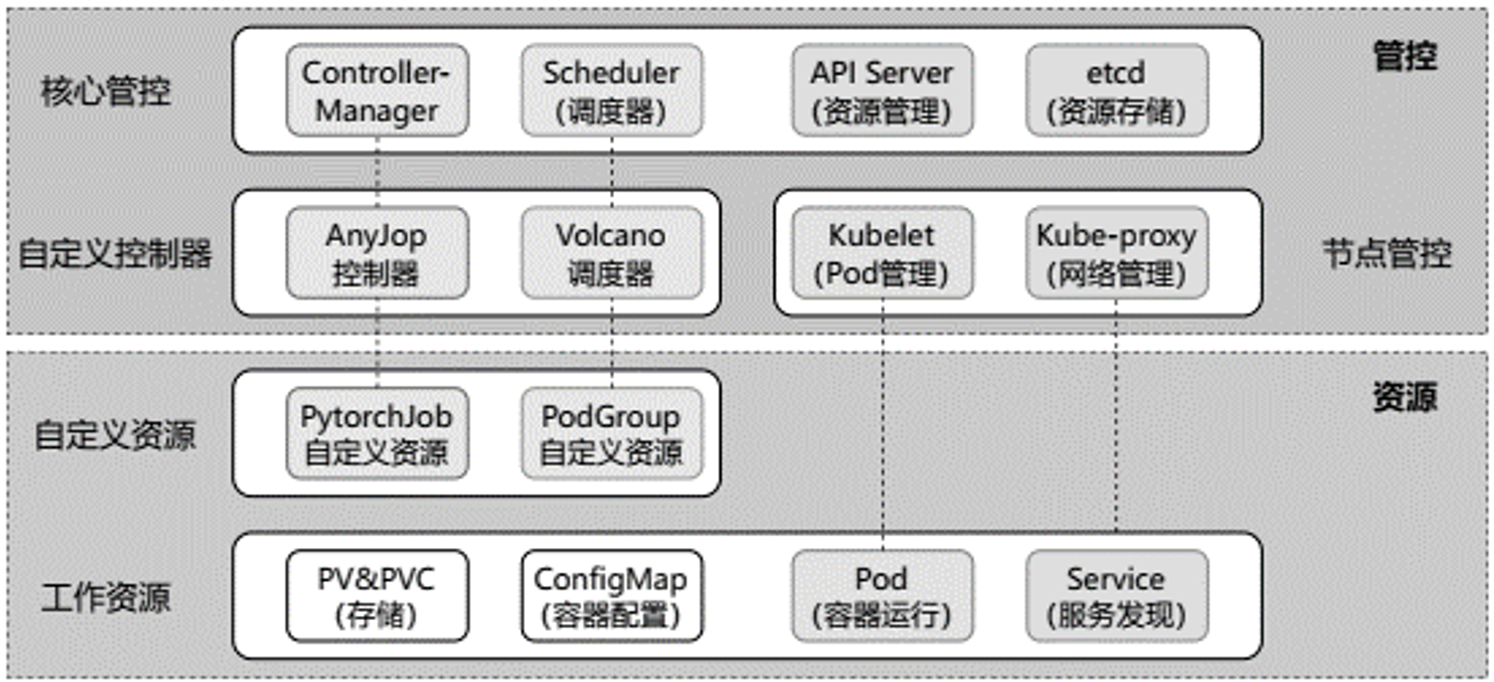
\includegraphics[width=0.8\linewidth]{dist-training-on-k8s.png}
  \caption{云原生分布式训练引擎基础架构示意}
  \label{fig:disttrainingk8s}
\end{figure}


\section{训练过程数据跟踪与可视化}

对于机器学习模型研发而言,训练过程的数据跟踪与可视化是非常重要的环节,能够帮助开发者更好地理解模型的训练过程,发现模型训练中的问题,提高模型的训练效率。
本节就训练过程数据跟踪与可视化的相关技术进行介绍。

\subsection{背景问题}

随着数据量和计算能力的不断提升,机器学习模型的训练过程变得更加复杂和耗时。
训练过程中的数据量大、计算密集度高,导致训练任务的管理和优化成为一项重大挑战。
当前,许多研究团队面临以下几个问题:

\textbf{(1)训练过程监控困难}

在深度学习模型的训练过程中,实时监控模型指标(如损失、准确率、梯度、权重等)对于研究人员来说至关重要。
这些数据能够帮助研究人员及时了解模型的训练状态,从而判断模型是否存在过拟合、欠拟合或训练效率低下等问题,并据此调整训练策略,优化模型性能。

目前,许多研究团队使用TensorBoard等开源工具来实现训练过程的监控。
TensorBoard提供了基本的可视化功能,但在某些方面存在局限性。
其中最显著的是,TensorBoard的多任务对比功能有限,它只允许对比同名指标,缺乏灵活性。
在实际研究中,研究人员常常需要对比不同模型或任务的多种指标,这就使得TensorBoard的功能显得不够灵活。

此外,TensorBoard的面板(panel)是固定的,用户无法根据不同任务和需求自定义面板。
这导致研究人员在需要展示特定指标组合时,往往需要下载数据并通过其他工具手动绘图,这无疑增加了操作的复杂性和工作量。
例如,假设研究人员正在同时训练两个模型,他们可能希望对比两个模型的准确率和损失。
但由于TensorBoard的多任务对比功能有限,他们可能无法直接在同一个界面中对比这两个指标。
他们可能需要打开两个不同的TensorBoard窗口,分别查看两个模型的指标,这样的操作显然不够便捷。
同样,如果研究人员希望自定义一个面板,以展示特定指标的组合,他们也将面临困难。
由于TensorBoard的面板是固定的,他们无法根据自己的需求来定制面板。
他们可能需要将数据导出到其他工具,如Matplotlib,然后手动绘制图表,这无疑增加了工作量。

总的来说,尽管TensorBoard是一个强大的可视化工具,但在多任务对比和自定义面板方面,它还存在一些局限性。
研究人员需要寻找其他工具或方法来满足这些需求。

\textbf{(2)数据分散管理}

在深度学习模型的训练过程中,数据的多样性和分散性带来了管理上的挑战。
训练过程中会产生多种类型的数据,如训练日志、模型权重、评估指标和训练数据等,这些数据通常分散存储在本地文件系统、远程服务器和云存储等多个位置。
这种分散管理的方式导致了数据读取效率低下,研究人员在分析和处理数据时需要频繁地在不同存储位置之间切换,从而增加了时间成本。
同时,数据一致性问题也随之产生,因为分散存储的数据可能会在不同位置出现版本不一致的情况,这会给研究人员在分析数据时带来困扰。

此外,数据的安全和隐私保护也面临着更大的挑战,因为数据存储在不同的位置,增加了泄露和丢失的风险。
缺乏集中管理的机制使得数据的安全性和隐私性难以得到有效保障。
在团队协作方面,分散的数据管理也增加了协同工作的难度,团队成员在需要访问和处理相同数据时,数据的传输和共享变得复杂,这影响了团队的整体工作效率。

为了解决这些问题,亟需开发一个高效的训练过程监控与数据管理系统,以克服现有工具的局限性。
这样的系统将实现数据的集中管理和高效处理,提升模型训练的管理和优化效率,同时确保数据的安全性和隐私保护,简化团队协作流程,从而推动研究工作的顺利进行。

\subsection{训练过程跟踪系统架构}

系统主要由交互层、业务层和存储层三个部分组成,如图\ref{fig:anyboardarch}所示。

\begin{figure}
  \centering
  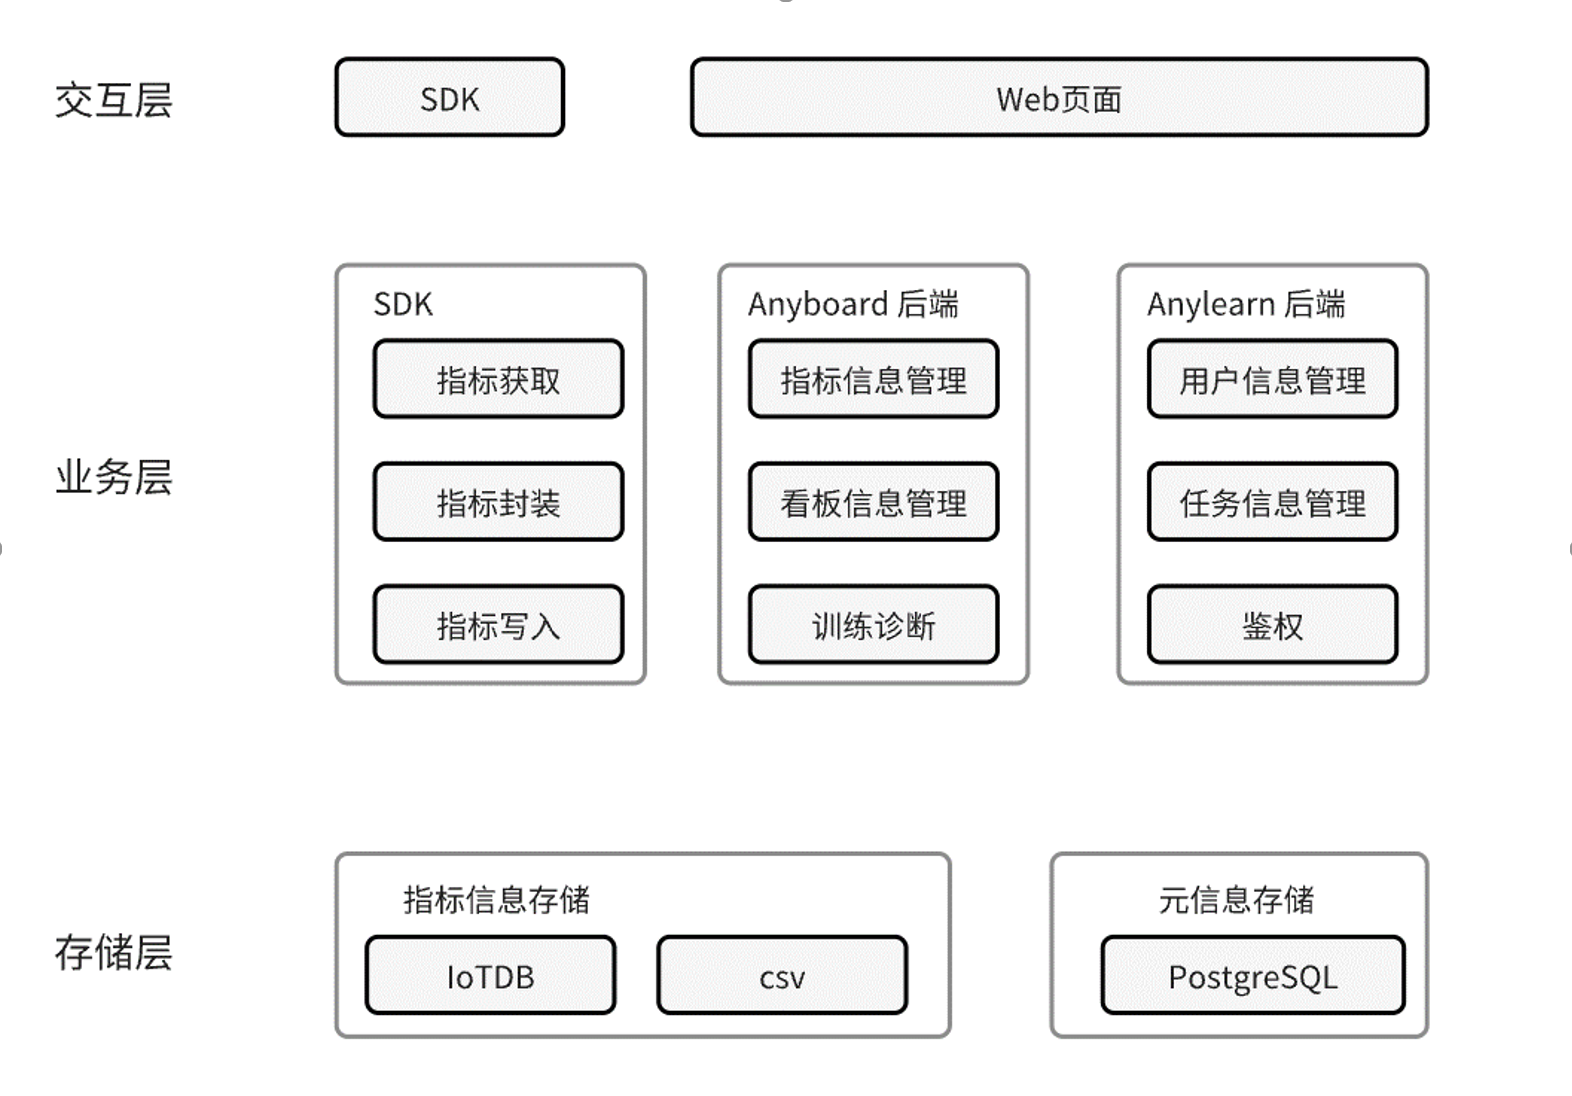
\includegraphics[width=0.8\linewidth]{anyboard-architecture.png}
  \caption{训练跟踪与可视化系统架构}
  \label{fig:anyboardarch}
\end{figure}

(1)交互层:首先,SDK作为编程接口,使用户能够在代码中直接记录训练过程中的各种指标数据。
它提供了方便的API,支持多种指标类型的记录,如标量、图片、直方图等。
通过SDK,用户可以在训练过程中方便地收集和记录所需的指标数据,以便后续分析和优化。
其次,Web页面通过直观的界面与用户交互,提供指标的实时可视化功能。
用户可以在Web页面上查看和分析训练过程中记录的各种指标数据。
Web页面将指标数据以图表、图像等形式展示给用户,使用户能够更直观地了解训练过程,发现潜在问题,并进行相应的调整和优化。
用户可以在Web页面上查看和分析训练过程中记录的各种指标数据。

(2)业务层:首先,指标记录功能处理用户通过SDK传入的指标数据。
当用户在代码中记录训练指标时,SDK将这些数据转换为标准格式,以确保数据的统一性和可处理性。
随后,这些标准格式的数据会被存储到后端数据库中,以便于长期保留和分析。
其次,指标管理功能负责管理和维护指标数据。
这包括创建新的指标数据记录、更新现有指标数据的值以及删除不再需要的指标数据。
指标数据的元信息,如指标名称、类型、单位等,也会被一同管理和维护,确保数据的准确性和完整性。
接着,指标展示功能提供实时数据查询和展示服务。
它将存储在数据库中的指标数据通过可视化的方式呈现给用户,例如以图表、曲线图或直方图的形式。
这样的展示方式帮助用户直观地理解训练过程,包括模型的性能变化、训练速度等关键信息。
最后,训练诊断功能基于记录的指标数据,对训练过程进行分析,以识别可能的异常情况。
它提供实时的诊断服务,帮助用户快速定位和解决问题。
例如,如果发现训练过程中的性能指标突然下降,诊断工具可以帮助用户分析造成这种情况的原因,是数据问题、模型结构问题还是学习率设置不当等。

(3)存储层:IoTDB时序数据库\cite{Wan23}专为存储时间序列数据设计,它在训练过程中用于收集和存储大量的时间序列数据。
时间序列数据是指按时间顺序记录的数据点集合,常用于监控系统性能、日志记录、气象数据等。
IoTDB支持高效的数据插入和查询操作,能够处理高频率、大规模的数据流,非常适合于训练过程中产生的海量时间序列数据的存储和管理。
IoTDB的特性包括数据压缩、数据索引、时间范围查询等,这些特性能够提高数据存储的效率和查询的速度。
CSV文件则适用于存储小规模离线训练任务的指标数据或作为数据文件的备份。CSV(Comma-Separated Values)文件格式是一种简单的文本文件格式,其中数据以行和列的形式存储,每列之间的分隔符通常是逗号。
CSV文件格式易于读取和处理,可以使用多种编程语言和工具进行数据的读取和分析。
对于小规模的训练任务,使用CSV文件存储指标数据可以快速方便地存取数据,而不需要复杂的数据库管理系统。
PostgreSQL是一种功能强大的关系型数据库,它用于存储训练过程中的元数据。元数据包括用户信息、项目信息和看板配置信息等。
这些信息通常是结构化的,需要进行复杂查询和事务处理。
PostgreSQL支持SQL查询语言,提供了高级的数据管理和操作功能,如数据完整性约束、视图、索引等。
使用PostgreSQL存储元数据可以确保数据的安全性、完整性和一致性,同时也便于进行复杂的数据分析和报告。

\subsection{端云协同的指标跟踪机制}

在端侧,通过SDK接口,用户可以在训练代码中直接记录指标数据,这极大地方便了数据的收集,并确保了数据记录的实时性和准确性。
同时,端侧的Web页面提供了直观的交互界面,使得用户能够实时查看训练指标,并通过图表等形式进行数据分析。

在云侧,采用了专业的时序数据库IoTDB来存储大量的时间序列数据,确保了数据的高效存储和快速检索。
此外,使用PostgreSQL数据库存储结构化元数据,提供了数据的安全性和复杂查询的支持。
云端的存储解决方案,不仅支持大规模数据的处理,还可以通过远程访问,实现数据的集中管理和分析。

系统的端云协同工作模式,允许用户在本地进行实时的数据监控和诊断,云端则负责长期的数据存储、分析和复杂查询。
这种工作模式使得用户能够充分利用本地资源进行快速开发和调试,同时又能够享受到云端强大数据处理能力和分析服务。
例如,当训练过程出现异常时,系统不仅能够实时检测到异常,还能够通过云端的大数据分析,为用户提供针对性的解决方案。

\subsection{实时数据展示与诊断}

实时数据展示与诊断是深度学习训练过程中的重要环节,它通过前端看板和相应的分析功能,使用户能够实时监控训练进度,快速识别和解决问题。

前端看板是实现训练指标实时可视化的界面。
它利用Vue框架和Echarts库,将训练过程中的各类指标以图表、曲线图、柱状图等形式展示给用户。
这些可视化元素使得训练过程中的复杂数据变得直观易懂,用户可以实时关注到模型的性能变化、训练速度、资源消耗等关键指标。
自定义面板功能允许用户根据不同任务的需求,灵活创建和配置看板。
用户可以根据自己的关注点,选择展示特定的指标,或者按照任务类型进行指标分类。
此外,自定义面板还支持多任务对比,帮助用户分析不同模型或任务的训练效果,从而做出更合理的决策。

训练诊断功能包括异常检测和问题解决建议两个部分。
异常检测是基于记录的指标数据,对训练过程进行实时分析,以发现可能的问题。
例如,系统可以检测梯度异常、损失变化异常等,这些异常可能是模型过拟合、学习率设置不当等原因造成的。
系统提供实时的诊断功能,帮助用户快速发现和定位这些异常。当检测到异常时,系统会提供相应的解决建议。
这些建议基于训练过程中的数据分析,旨在帮助用户及时调整训练策略,优化模型性能。
例如,如果检测到梯度消失问题,系统可能会建议尝试调整学习率或使用更合适的优化器。
通过上述技术原理,系统实现了对训练过程的高效监控和数据管理,解决了现有工具的局限性,显著提升了训练任务的管理和优化效率。


\section{超参数高效调优}

超参数调优往往对机器学习模型的效果起着决定性的作用,在模型应用落地时至关重要。
本节就高效超参数调优技术进行介绍。

\subsection{背景问题}

深度神经网络(DNN)在许多应用中取得了显著的成功,特别是在图像识别、自然语言处理、语音识别等领域。然而,DNN的性能高度依赖于超参数的选择,合理的超参数设置能够显著提升模型的表现。然而,传统的超参数调优方法面临以下几方面的挑战。

(1)超参数组合多:深度神经网络(DNN)的超参数种类繁多,包括学习率、批量大小、网络层数、每层的神经元数量、激活函数的选择、正则化参数等。
每种超参数都有多个可能的取值,例如,学习率可以是0.001、0.01或0.1,批量大小可以是32、64或128,网络层数可以是3层、5层或10层,激活函数可以选择ReLU、Sigmoid或Tanh,正则化参数可以是L2正则化、Dropout等。
由于每个超参数的可能取值都不同,所有可能的组合数量呈指数增长。
例如,如果有6种超参数,每种超参数有3个可能取值,组合数将是3的6次方,即729种组合。
这种组合数量随着超参数数量和每个超参数的取值范围的增加而迅速增长,使得全面搜索所有可能的超参数组合变得几乎不可能。
此外,实际应用中,为了获得最优的DNN模型,往往需要尝试更多种类的超参数及其更多的取值,这进一步增加了组合数量的复杂性和计算量,给传统的超参数调优方法带来了巨大挑战。
这种组合爆炸现象严重影响了超参数调优的效率和效果,导致计算资源浪费和调优过程的冗长。

(2)训练耗时长:每次对超参数组合的评估都需要进行完整的训练和验证过程,这在大规模数据集和复杂模型结构下尤为耗时。
深度神经网络通常包含数百万甚至数十亿个参数,这些参数需要通过反复的前向传播和反向传播来优化。
对于大型数据集,每次训练迭代都需要处理大量的数据,这使得训练时间大幅增加。
此外,复杂的模型结构,如深度较大的卷积神经网络(CNN)或包含大量节点的循环神经网络(RNN),需要更多的计算资源来完成每次迭代。
因此,训练一个模型可能需要数小时、数天甚至数周的时间。
当进行大规模的超参数调优时,需要对大量不同的超参数组合进行试验,每个组合都需要完整的训练和验证过程,这进一步加剧了耗时问题。
这种大规模的训练需求耗费了大量的计算资源和时间,严重限制了调优效率。
即使使用高性能计算设备,如GPU或TPU,加速效果也有限,因为每次超参数调整都需要重新开始训练过程。
由于超参数空间巨大,传统的网格搜索或随机搜索方法需要尝试数百甚至数千种组合,这使得超参数调优过程变得异常缓慢和昂贵,无法快速找到最佳的超参数组合,从而影响了模型性能的优化。

(3)训练过程随机性大:深度神经网络(DNN)的训练过程具有高度的随机性,这源于多个方面的因素。
首先,权重初始化的随机性在训练开始时就引入了不确定性,不同的初始化可能导致模型收敛到不同的局部最优解。
其次,数据的随机分批处理(mini-batch)在每个训练迭代中使用的数据子集是随机选择的,这种随机选择会影响模型参数的更新路径。
此外,优化算法中的随机性,如随机梯度下降(SGD)及其变种(如Adam、RMSprop),在每次参数更新时都会引入随机噪声,从而影响模型的收敛过程。
这些随机因素的综合作用导致同一组超参数在不同的训练过程中可能得到显著不同的结果,表现为模型性能的波动。
这种结果的不一致性增加了超参数调优过程的不确定性和难度,因为无法确定某次试验结果的优劣是由超参数本身决定的,还是由训练过程的随机性导致的。
为了克服这些随机性影响,需要多次重复试验并取平均值或最优值来评估超参数组合的性能,这进一步增加了计算成本和时间开销。
随机性的存在还使得超参数调优结果的可重复性和稳定性降低,使得调优过程变得更加复杂和耗时。

这些问题严重影响了DNN超参数调优的效率和效果。
传统方法如网格搜索(Grid Search)和随机搜索(Random Search)虽然简单直观,但面对高维度超参数空间和训练时间长的问题时显得无力。
针对这些挑战,需要开发新的技术手段,以更高效、更精准地进行超参数调优,从而提升深度神经网络的性能和应用价值。

\subsection{基于训练诊断的超参数调优}

为了应对上述挑战,学界提出了一种基于训练时学习过程质量指标的超参数调优方法\cite{Pei24}。
该方法的核心思想是通过实时监测和评估训练过程中的质量指标,提前停止那些表现不佳的超参数组合试验,节约计算资源并将其用于更有潜力的组合。

技术架构如图\ref{fig:anytunerarch}所示,主要包括指标监测模块、质量评价模块和资源调度模块三个部分。

\begin{figure}
  \centering
  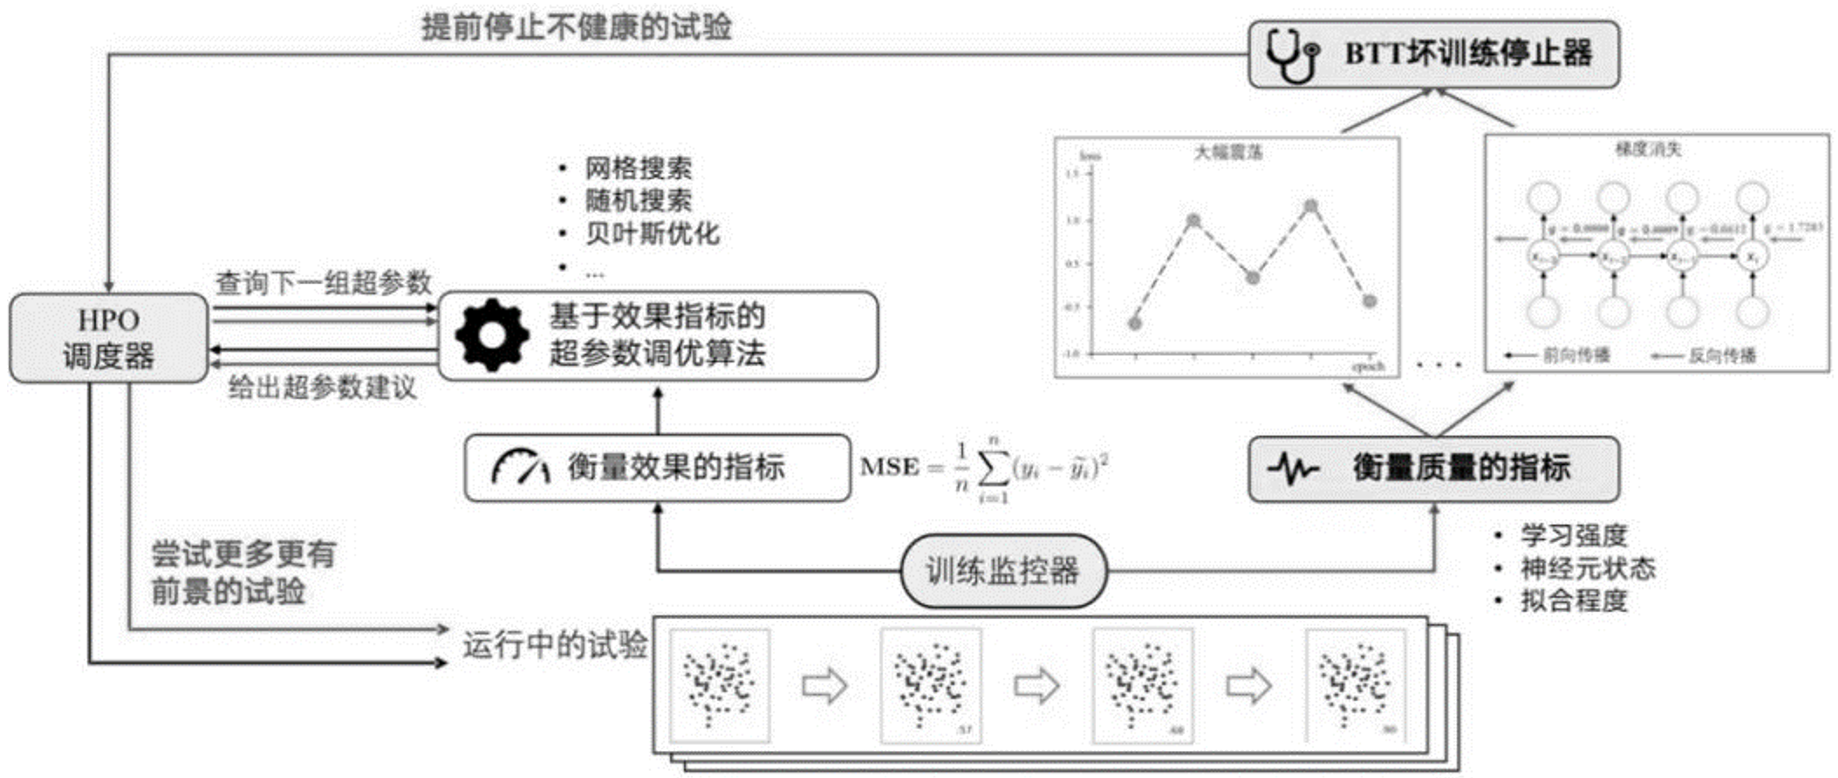
\includegraphics[width=0.8\linewidth]{anytuner-architecture.png}
  \caption{基于训练诊断的超参数调优系统架构}
  \label{fig:anytunerarch}
\end{figure}

(1)指标监测模块:实时监测训练过程中的质量指标,如损失函数值、准确率等。

该模块负责实时监测训练过程中的各种质量指标,如损失函数值、准确率、验证集表现等。
在每个训练迭代中,记录关键指标的变化趋势,并对比历史记录,分析当前超参数组合的性能。
具体实现方式包括在每个训练迭代中,实时记录训练集和验证集的损失函数值和精度,分析其变化趋势。
数据采集通过深度学习框架(如TensorFlow、PyTorch等)的钩子(hook)机制进行,采集训练过程中每个batch的指标数据。
监测内容不仅限于训练集和验证集的损失函数值、训练精度和验证精度,还包括梯度范数、学习率变化等。
具体收集的指标还包括高维度的模型参数值和梯度值的统计量(如中位数、平均值、最大值、方差、四分位数、偏斜值等),以及模型结构信息。
这些指标的收集和分析有助于判断训练过程中的过拟合、欠拟合或训练不稳定等问题。
例如,梯度范数的异常变化可能表明存在梯度爆炸或消失的问题,学习率变化的监控可以帮助识别是否需要调整学习率策略,参数值的统计量则可以揭示模型训练的健康状态。
通过这些措施,能够实时了解和评估每个超参数组合的训练效果,为后续的质量评价和资源调度提供准确的数据支持。

(2)质量评价模块:根据预设的评价标准,对当前超参数组合的训练质量进行评价。

该模块基于预设的评价标准对当前超参数组合的训练质量进行实时评价。
具体实现方式包括采用一系列评价标准,例如提前停止标准、稳定性标准和进展标准。
提前停止标准是指如果在一定的训练迭代内,验证集损失函数未能显著降低,则判定为预期效果不佳。
稳定性标准监测损失函数的波动情况,若波动过大且未能收敛,视为质量不稳定。
进展标准则结合学习率调整策略,评估模型在不同学习率下的表现,判断当前超参数组合的有效性。
评价流程通过设定阈值和规则,自动化地对训练过程中的指标进行分析,生成评价报告。
评价标准设置方面,根据不同任务的需求,设定具体的评价标准和阈值。
例如,损失函数收敛性可以设置为若损失函数在连续若干迭代中下降幅度小于预设阈值,则判定为收敛性不佳;
验证集表现标准则为若验证集损失在一定迭代数内未显著降低,或验证集精度无明显提升,则判定为效果不佳。
通过这些预设的评价标准,模块能够自动化地对每个超参数组合进行评价,生成实时评价报告,从而为后续的资源调度提供依据。

(3)资源调度模块:根据评价结果,提前停止那些预期效果差的超参数组合,并将释放的计算资源重新分配给其他有潜力的超参数组合进行训练。

该模块根据质量评价结果,进行计算资源的智能调度,提前停止那些预期效果差的超参数组合试验,并将释放的计算资源重新分配给其他有潜力的超参数组合进行训练。
具体实现方式包括任务调度器、任务终止器和资源再分配器。
任务调度器负责管理和分配计算资源,根据评价结果动态调整资源分配策略,确保高效利用计算资源。
任务终止器在判定某个超参数组合效果不佳后,及时停止其训练任务,避免资源浪费,并立即释放相应资源。
资源再分配器则将这些释放的资源重新分配给新的超参数组合或正在训练中的有潜力的组合,以加速其训练进程。
调度策略采用优先级调度策略,根据质量评价结果的优先级,灵活调整计算资源的分配,确保资源最大化利用。
通过动态任务调度,系统能够根据质量评价报告实时调整计算资源的分配策略,将资源优先分配给表现良好的超参数组合;
通过提前停止策略,及时终止预期效果差的超参数组合训练任务,避免资源浪费;
通过资源再分配策略,将释放的计算资源高效地重新分配给新的或潜力超参数组合,显著加速其训练过程,从而提高整体调优效率。

\begin{figure}
  \centering
  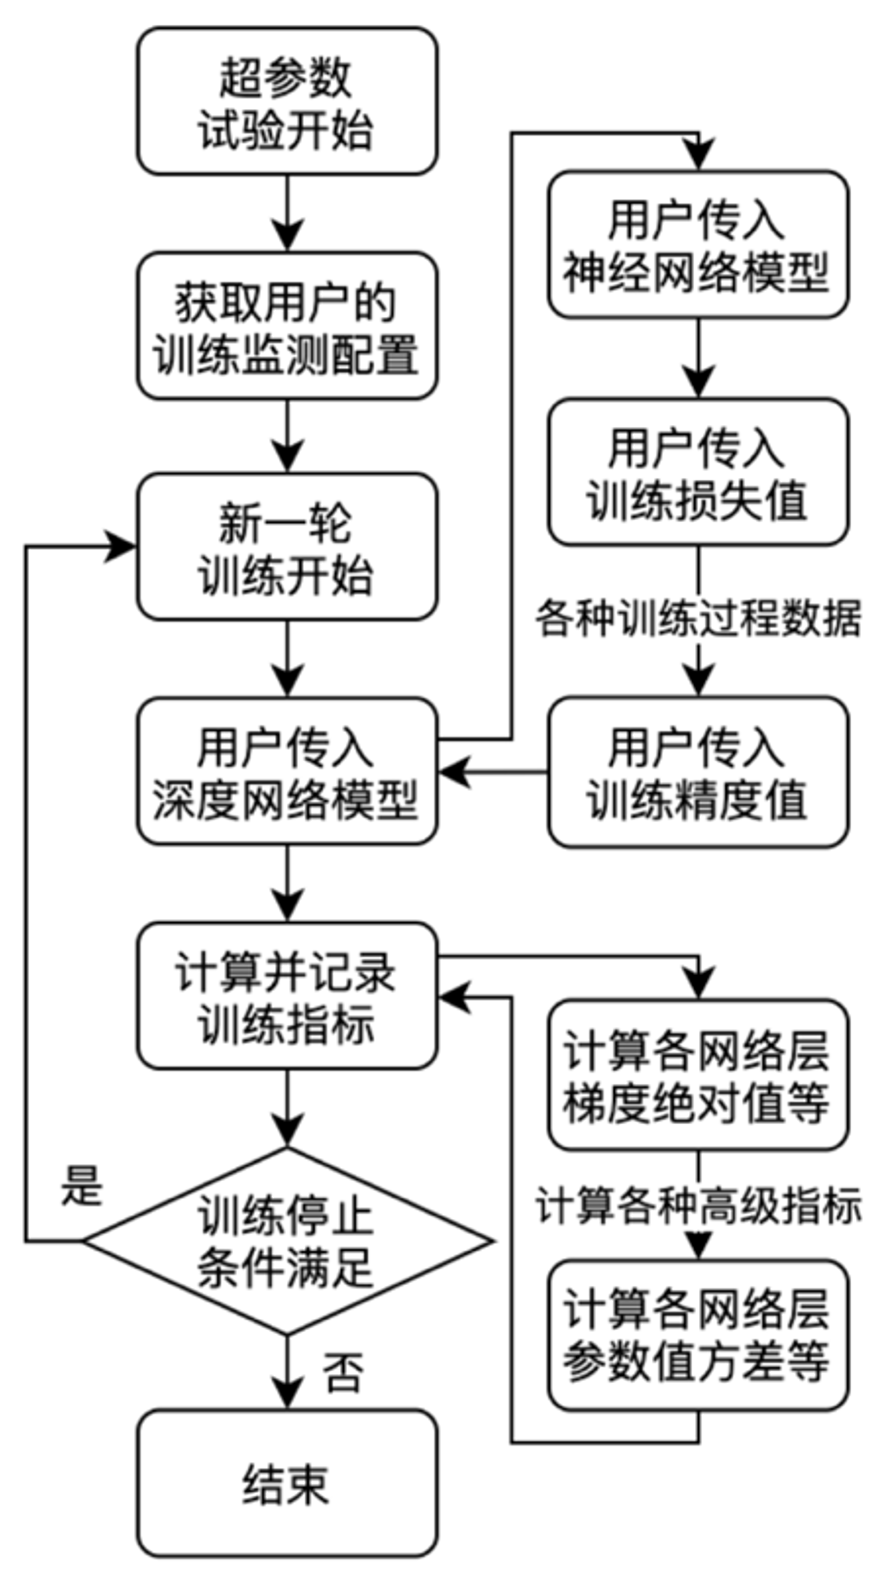
\includegraphics[width=0.3\linewidth]{anytuner-workflow1.png}
  \caption{基于训练诊断的超参数调优工作流程1}
  \label{fig:anytunerworkflow1}
\end{figure}

\begin{figure}
  \centering
  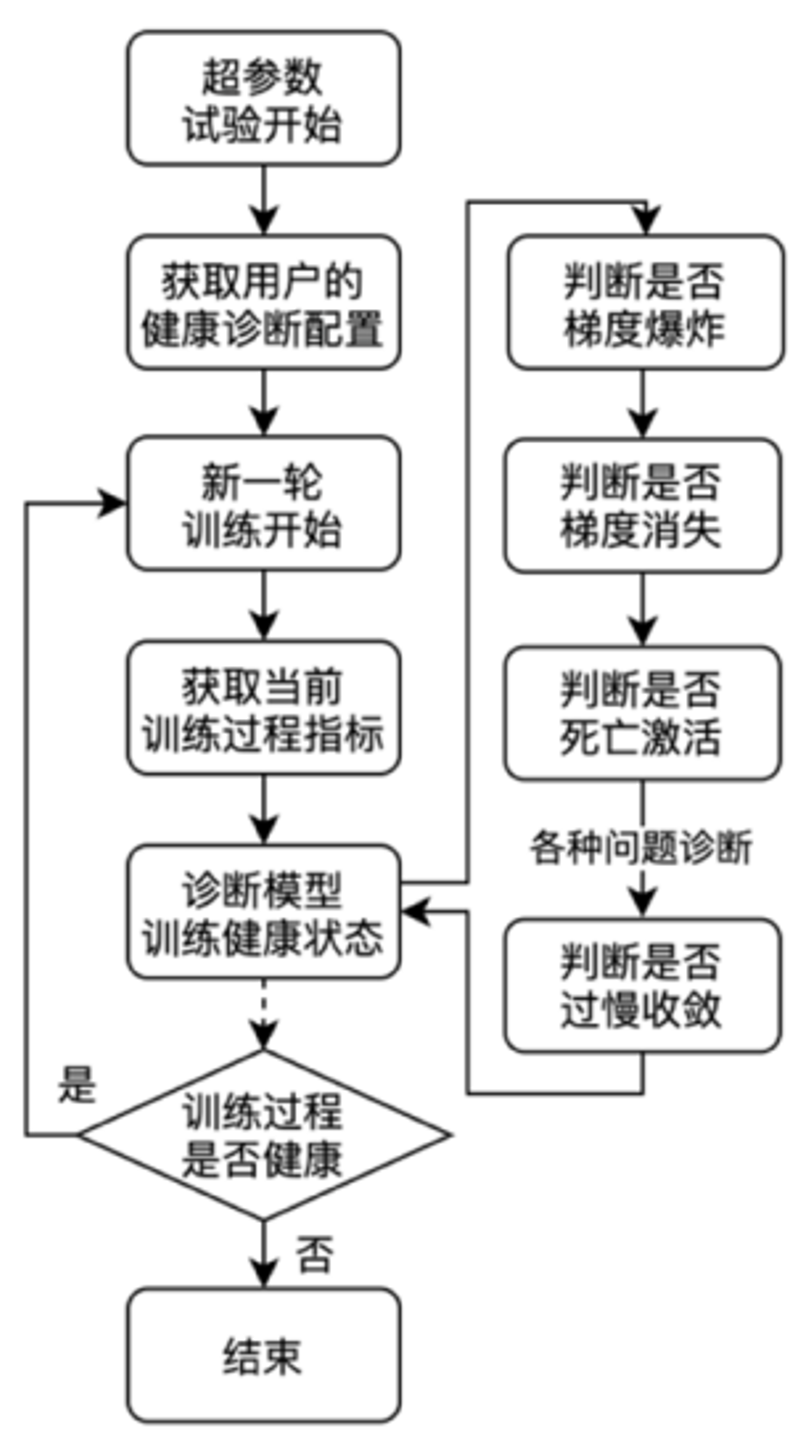
\includegraphics[width=0.3\linewidth]{anytuner-workflow2.png}
  \caption{基于训练诊断的超参数调优工作流程2}
  \label{fig:anytunerworkflow2}
\end{figure}

\begin{figure}
  \centering
  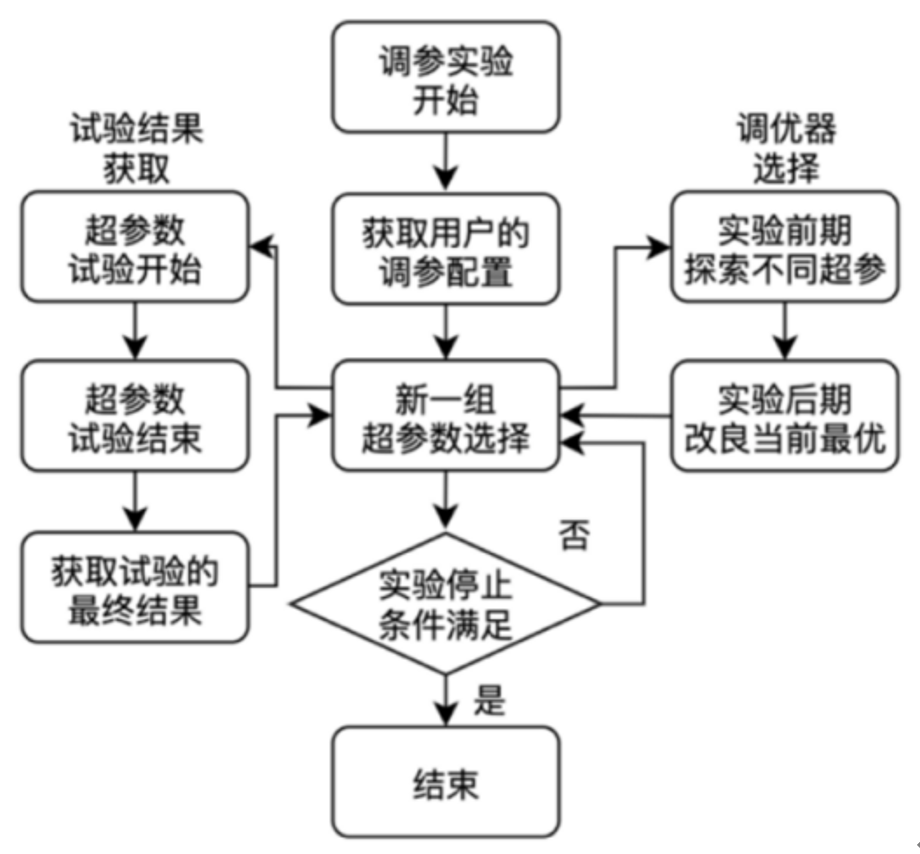
\includegraphics[width=0.5\linewidth]{anytuner-workflow3.png}
  \caption{基于训练诊断的超参数调优工作流程3}
  \label{fig:anytunerworkflow3}
\end{figure}

\subsection{实时质量监测和评价}

实时质量监测:传统的超参数调优方法通常需要等待一个完整的训练周期结束后,才能对超参数组合的效果进行评估。
这种方式的缺点在于,如果一个超参数组合的效果较差,那么只有等待该任务完全结束之后才能重新开始尝试新的组合,导致大量的计算资源浪费。
本技术方案通过实时监测和评价训练过程中的质量指标(如准确率、损失函数值等),可以在训练过程中及时识别和淘汰效果差的超参数组合。
这样,不仅可以减少无效的训练任务,还可以提高调优效率,加快模型的开发速度。

训练质量评价:该技术方案通过一系列预设的评价标准(如提前停止标准、稳定性标准、进展标准等),对当前超参数组合的训练质量进行实时评价。
利用这些评价标准,可以动态地对每个超参数组合的训练效果进行评估,从而在早期阶段就识别出表现不佳的组合,并及时停止这些组合的训练任务。
这种实时的质量评价方式能够有效地减少计算资源的浪费,并提高超参数调优的效率。

\subsection{资源高效利用和动态调度策略}

资源高效利用:在传统的机器学习模型调优过程中,通常会同时运行多个超参数组合的训练任务,以比较它们的效果。
然而,由于每个超参数组合的训练时间可能不同,导致计算资源的利用效率不高。
本技术方案通过提前停止无效训练试验,释放计算资源,并将其用于更有潜力的超参数组合。
具体来说,当一个超参数组合的训练效果已经明显劣于其他组合时,可以提前停止该组合的训练,并将计算资源分配给其他更有潜力的组合。
这样,可以显著提升计算资源的利用效率,加快模型的开发速度。

动态调度策略:传统的机器学习模型调优过程中,通常采用固定的资源分配策略,即每个超参数组合分配相同的计算资源。
这种方式的缺点在于,无法根据超参数组合的训练效果动态调整资源分配,导致资源利用不充分。
本技术方案基于实时评价结果,动态调整训练资源分配策略。
具体来说,当某个超参数组合的训练效果较好时,可以优先分配更多的计算资源给它以及和它相似的其他超参数组合,以加快其训练速度;
反之,当一个超参数组合的训练效果较差时,可以减少其计算资源分配,或者直接提前停止训练,以避免浪费。
通过这种方式,可以确保资源优先分配给预期效果较好的超参数组合,显著提升计算资源的利用效率,提升调优的效果和效率。


\section{大模型微调}

如今,大语言模型已广泛应用在多个领域,其核心能力在于能够根据用户私有数据进行微调,得到用户自有的大模型,以适应特定任务的需求。
本节将介绍大模型微调的技术原理和方法。

\begin{figure}
  \centering
  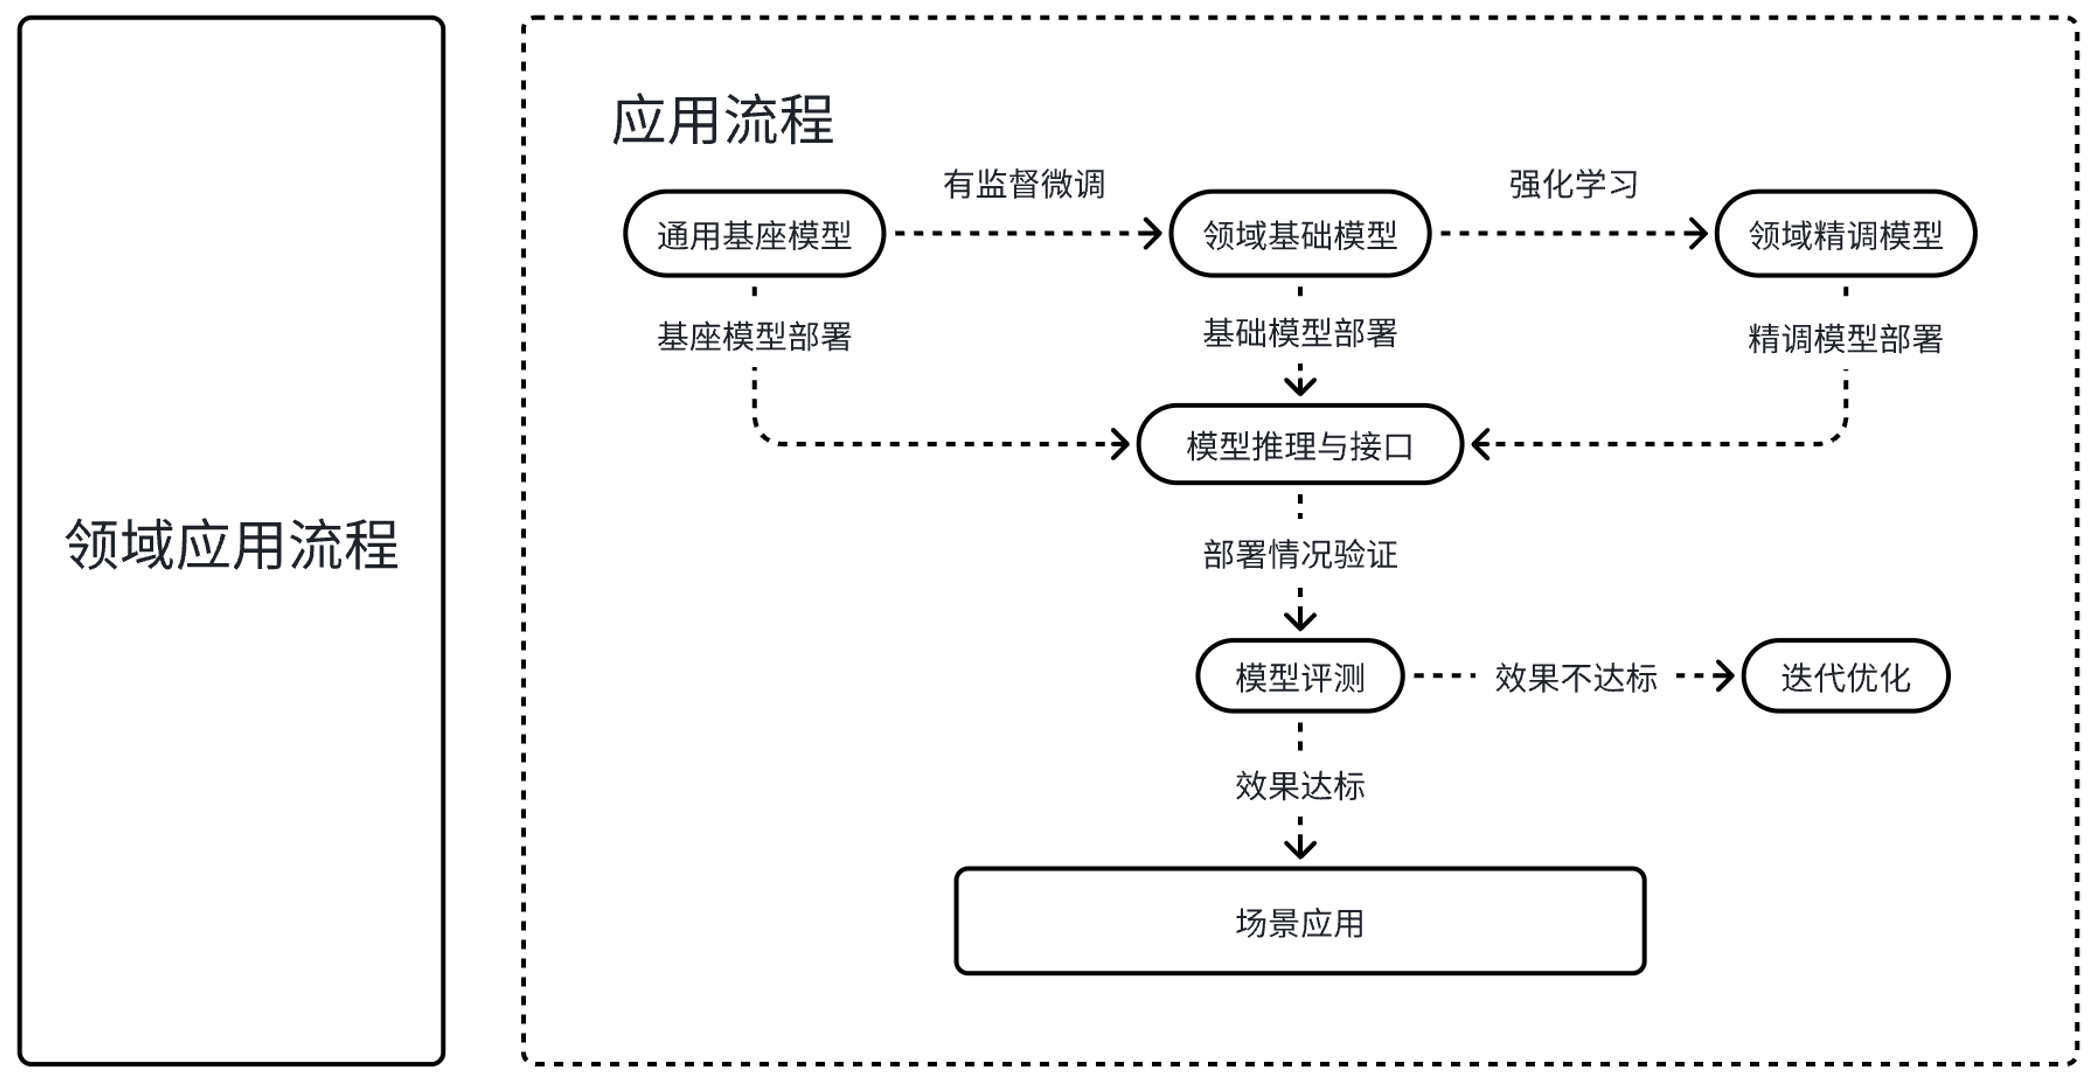
\includegraphics[width=0.8\linewidth]{llm-finetuning-overview.png}
  \caption{大模型微调领域应用流程概览}
  \label{fig:finetuning}
\end{figure}

\subsection{背景问题}

进行大模型微调需要大量的算力与数据作为支撑,是进行大模型微调研究者所需要解决的最基本问题。
微调过程与从头开始训练一个大型深度学习模型同样需要巨大的数据集和计算资源。
这不仅成本高昂,而且对于大多数组织和个人来说,获取和维护这样的资源是不切实际的。
同时,大型模型的参数量巨大,训练它们需要大量的时间和算力与高昂的电力和硬件成本。
另外,为了训练一个表现良好的模型,通常需要大量的标注数据。
在某些领域,获取足够的高质量标注数据是具有挑战性的,特别是对于特定任务或小数据集。

由于微调过程涉及到参数的进一步调整与优化,研究者需要时刻注意预训练任务与微调任务之间的兼容性。
当一个预训练模型在新任务上进行微调时,它可能会忘记之前学到的知识,这限制了模型在新任务上的表现。
尽管大型预训练模型在广泛的任务上表现出色,但它们可能并不完全适应特定的应用领域或特定类型的数据。
大模型微调过程需要尽可能地避免领域不适配带来的模型效果劣化,以最大程度发挥大模型预训练在微调任务上的潜力。

与传统的一次性训练小模型一样,大模型微调要求模型具有定制化的特征。
预训练模型无法覆盖所有应用场景,因此不同的应用场景需要模型针对不同的功能和特性进行定制化微调。
通过微调,可以使模型更好地适应特定领域的需求和特征。
在定制化微调过程中,研究者也希望模型能够保持安全性与泛化性,即在避免危险数据泄露的同时在多种任务上保持出色表现。

\subsection{大模型微调技术原理}

整体步骤上,大模型微调一般分为有监督微调与强化学习两个步骤。
第一,有监督微调使用标注过的数据来调整预训练模型的参数,使其更好地适应特定任务或领域,是较为经典的微调方法。
第二,强化学习模型通过将输入序列分布作为状态空间,将所有可能得token作为动作空间,将特殊设计的奖励模型的输出与策略约束作为价值函数,将大模型下一token选择累计奖励最大化作为策略函数,进一步增强大模型的能力。

微调方式上,大模型可通过全量调整所有参数以充分适应新任务,或采用参数高效微调技术仅优化部分参数以实现快速且低成本的迁移学习。
大模型全量微调随着模型体量的上涨而变得越来越昂贵,促成了参数高效微调技术的广泛探索。

然而,随着针对微调算法的探索不断深入,越来越多的大模型微调算法不断涌现出来。
对于不同的大模型微调任务,不同的算法有着差异化的表现。
如何选择基础模型、如何收集处理领域数据,如何在合适的场景下选择最优的大模型微调方式成为了重要的问题。
为了解决这些问题,我们提出设计一种大模型微调基座平台以加速基础模型、领域数据与微调算法之间的匹配。

\begin{figure}
  \centering
  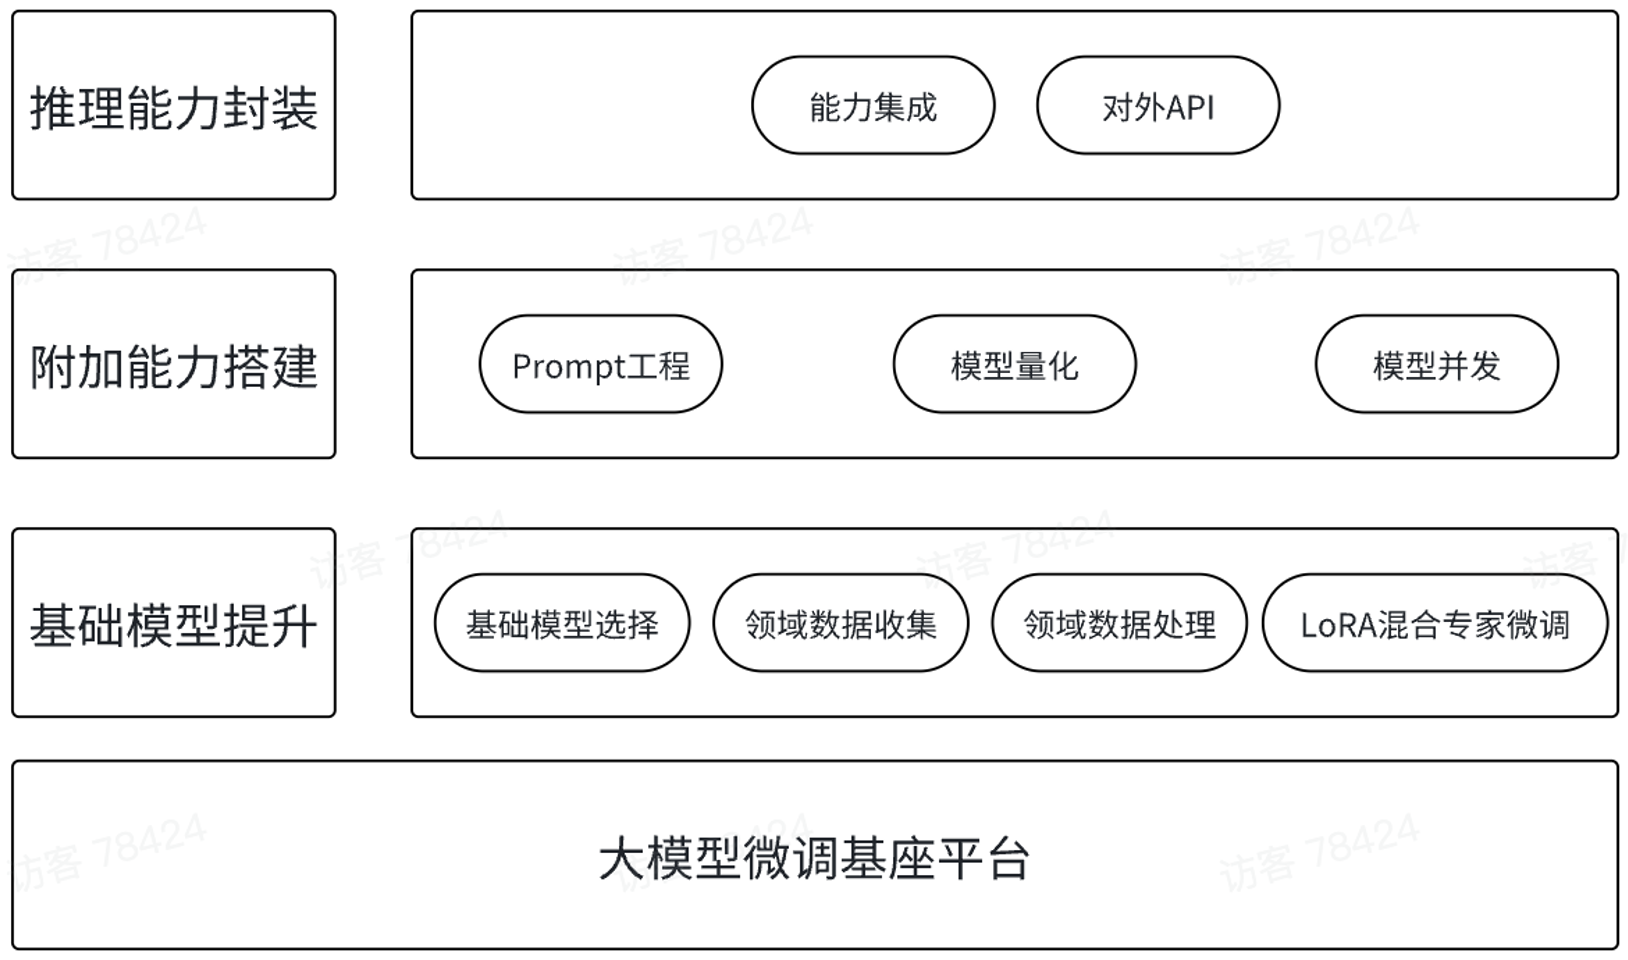
\includegraphics[width=0.8\linewidth]{llm-finetuning-system.png}
  \caption{大模型微调基座平台技术原理}
  \label{fig:finetuningsys}
\end{figure}

大模型微调基座平台包括基础模型提升、附加能力搭建与推理能力封装三部分。
首先,大模型微调基座平台可以通过集成基础模型选择、领域数据收集、领域数据处理与LoRA混合专家微调四个模块来提升基础模型能力。
基础模型选择模块通过在现有的比对指标上进行标准化测试以筛选当前表现较为出色的预训练基础大模型。
领域数据收集模块与领域数据处理模块负责制作用于微调过程的标准化数据,并嵌入任务语义与目标偏好。
最终,通过多种微调方法共同微调的方式使得大模型学习对应的任务语义与目标偏好,实现大模型微调流程。

其次,大模型微调基座平台可以通过Prompt工程、模型量化与模型并发等模块基于基础模型进一步搭建附加能力。
Prompt工程模块弥补了基础模型提升过程中对于目标任务理解偏差的问题,赋予模型通过Prompt理解具体任务需求的能力。
模型量化模块通过低精度浮点数计算进一步压缩了模型微调与推理的计算开销,赋予模型快速微调推理的能力。
模型并发模块通过在流水线、数据与模型权重等维度上的拆分,使得大模型在较小显存的显卡集群上也能有不俗的微调推理表现,赋予模型在低计算资源配置情景下的使用能力。

最终,大模型基座平台可以通过能力集成与对外API模块实现云端的快速部署。
能力集成模块基于面向对象编程思想,将平台的全部功能进行必要的合并与拆分,形成针对大模型微调场景的函数工具箱。
对外API模块将基座平台的主要功能以REST API等形式进行封装,主要负责基座平台对用户提供的云服务。

\subsection{混合专家系统}

混合专家系统(Mixture of Experts, MoE)是在神经网络领域发展起来的一种集成学习(Ensemble Learning)技术。
传统的深度学习模型在训练时,对于每个输入样本,整个网络都会参与计算。
随着模型越来越大,训练使用的样本数据越来越多,训练的开销越来越难以承受。
而MoE可以动态激活部分神经网络,从而实现在不增加计算量的前提下大幅度增加模型参数量。

MoE 技术目前是训练万亿参数量级模型的关键技术。
MoE 将预测建模任务分解为若干子任务,在每个子任务上训练一个专家模型(Expert Model),开发一个门控模型(Gating Model),该模型根据要预测的输入来学习信任哪个专家,并组合预测结果。尽管该技术最初是使用神经网络专家和门控模型来描述的,但它可以推广到使用任何类型的模型。

\subsection{LoRA}

LoRA(Low-Rank Adaptation)是一种旨在微调大型预训练语言模型(如GPT-3或BERT)的技术。
其核心理念在于,在模型的决定性层次中引入小型、低秩的矩阵来实现模型行为的微调,而无需对整个模型结构进行大幅度修改。
这种方法的优势在于,在不显著增加额外计算负担的前提下,能够有效地微调模型,同时保留模型原有的性能水准。

由于LoRA的出色性能,部分工作尝试对LoRA进行升级改进。
QLoRA(Quantized Low-Rank Adaptation)是一种结合了LoRA(Low-Rank Adaptation)方法与深度量化技术的高效模型微调手段。
这种方法采用创新的技术将预训练模型量化为4位,包括低精度存储数据类型(4-bit NormalFloat,简称NF4)和计算数据类型(16-bit BrainFloat),极大地减少了模型存储需求,同时保持了模型精度的最小损失。

与LoRA技术类似,适配器调整(Adapter Tuning)的目标是在保留预训练模型原始参数不变的前提下,使模型能够适应新的任务。
适配器调整的方法是在模型的每个层或选定层之间插入小型神经网络模块,称为“适配器”。
这些适配器是可训练的,而原始模型的参数则保持不变。

LoRA混合专家微调同样遵循混合专家模型的一般流程。用于训练多个模型以解决复杂任务的技术。
大模型微调基座平台会针对不同的任务和数据,选择特定数量的LoRA来充当专家模型。具体流程如下:

(1)准备搜集数据:
收集和准备用于训练的数据集。数据集应该包含输入特征和对应的目标值(或标签),以及特定LoRA标识。
需要知道哪个任务应该由哪个专家模型处理。

(2)选择专家(LoRA)数量:
决定使用多少个专家模型。
这通常根据任务的复杂性和数据集的规模来选择。
专家数量可以根据经验进行调整,也可以通过交叉验证等方法选择。

(3)初始化专家(LoRA)模型:
初始化每个专家模型的参数。
可以使用随机初始化或者预训练模型来初始化。
这边的LoRA是随机初始化的。

(4)训练专家(LoRA)模型:
根据特定任务为每个LoRA模型分别训练参数。
这通常是标准的模型训练过程,使用输入特征和对应的目标值来更新模型参数。
可以使用梯度下降等优化算法进行参数更新。

(5)训练门控模型(Gating):
门控模型的标签实际上是每个输入对应的专家模型的标识。
门控模型通过学习输入特征与对应的专家模型之间的关系,来决定选择哪个专家模型来处理输入。
训练过程的目标是最小化分类误差,使门控模型能够准确地选择适当的专家模型。

(6)前向传播和损失计算:
将输入特征通过专家模型和门控模型进行前向传播,得到每个专家模型的预测结果和门控模型的预测结果。
然后,计算损失函数,该损失函数包括专家模型的损失和门控模型的损失。

(7)反向传播和参数更新:
使用反向传播算法计算整个Mixture of LoRA模型的梯度,并更新所有模型的参数,包括专家模型和门控模型。

(8)迭代训练:
重复训练过程,多次迭代更新参数,直到模型收敛或达到预定的训练迭代次数。

(9)评估和调优:
使用验证集或测试集来评估模型性能,根据性能表现进行调优,可以调整专家数量、门控模型的结构、训练参数等。


\section{模型更新}

模型开发完成后,集成进入业务系统生产环境,持续接入真实业务数据并进行推理。
然而,真实数据与训练数据之间客观存在的分布差异会导致模型效果随时间推移而下降,需要及时更新模型以保持模型的性能。
本节就模型更新的相关技术进行介绍。

\subsection{背景问题}

机器学习模型的一种常见的开发和应用流程大致是,开发者首先面向目标场景设计出一套机器学习算法或是直接选用现成算法,接着准备一定量的能够代表目标场景的数据(即训练集),然后用准备好的算法在准备好的训练集的基础上训练出表现良好的模型,最后再把训练好的模型部署到生产环境。
根据机器学习的理论,在线下表现良好的模型在线上也能表现良好的一个前提是,模型在线上所接触到的数据与用来训练该模型的数据服从相同的统计分布,而这个前提在现实中却经常会被打破。
在现实场景中,各种各样的因素都会带来线上数据分布随时间变化进而偏离训练集数据分布的结果,业界把这种线上数据分布随时间变化的现象称为数据偏移。

应对数据偏移问题的一种直接的思路是,首先通过某种方法来检测潜在的数据偏移(即偏移检测),在检测到数据偏移后再通过某种方法来更新模型以让模型适应新的数据分布(即偏移适配)。
大多数偏移检测方法监视模型预测效果随时间的变化,在模型效果的下降具有统计显著性时汇报偏移,我们把这类方法称为基于模型效果的偏移检测方法;
除此之外,也有一些偏移检测方法选择直接监视输入数据分布随时间的变化,我们把这类方法称为基于输入分布的偏移检测方法,这类方法相比基于模型效果的偏移检测方法的优点在于不需要线上数据的真实标签就能够工作(评价模型预测效果需要真实标签),但也存在计算成本过高和敏感度过高等问题。
至于偏移适配,最通用的偏移适配方法是用属于新分布的数据来训练新模型取代旧模型;
除此之外,也有一些模型相关的偏移适配方法被提出。
除了先做偏移检测再做偏移适配,还有一种思路是直接做偏移适配,这类偏移适配方法包括一些基于集成学习的方法,它们隐含了感知数据偏移的能力,会依据新到来的数据持续更新模型,不需要与专门的偏移检测方法配合使用。
为方便后面叙述,我们把包括上述方法在内的为解决数据偏移问题而提出的方法统称为偏移对策。

尽管目前已经有很多种偏移对策,但对不熟悉数据偏移领域的研发人员来说,把这些对策应用于实际场景仍然存在困难。

不同的对策和这些对策的不同参数取值(以下合称对策)所适用的数据偏移场景(如渐替偏移的渐替速率、是否存在概念重现)是不同的。
为了给目标场景选取合适的对策,研发人员不但需要对多种对策以及它们的工作机制有所了解,还需要对目标场景的数据偏移特性有所认识,这就给研发人员带来了使用门槛。

即使研发人员有能力为目标场景选取合适的对策,也还面临在生产环境中合理使用所选对策的难题。
生产环境中往往存在一些复杂的情况,例如输入数据的真实标签可能延迟到来、乱序到来甚至缺失,或是模型更新期间可能仍有新的输入数据到来,等等。
为此,研发人员需要为模型和偏移对策设计和实现合理的实际运行逻辑。
这里的难点有两个,一是研发人员需要周全考虑生产环境中的各种可能情况以免造成意外后果,二是合理的实际运行逻辑将涉及历史数据的暂存和异步维护,这要求研发人员具有一定的多线程编程能力。

即使研发人员有能力为模型和偏移对策设计和实现合理的实际运行逻辑,也还面临在部署之前评测所选偏移对策的难题。
评测本质上是对实际运行过程的模拟,其难点在于确保逻辑与实际运行等价的同时尽可能地节省时间。
目前也有一些现成的偏移对策评价方法,但这些方法并不满足逻辑与实际运行等价的条件(因为它们并非是针对某种模型和偏移对策实际运行逻辑开发出来的),而且往往对生产环境的情况做了较大的简化,因此这些方法所给出的评价结果不一定能符合生产环境的情况。

\subsection{模型更新策略评价}

为降低研发人员把现有偏移对策应用于实际场景的门槛,本技术将帮助研发人员构造具有数据偏移自适应能力的模型服务。

技术主要流程如下图所示,分构造和运行两个阶段。
在构造阶段,研发人员首先以“手动”或“自动”的方式构造模型更新策略,即偏移检测器和模型更新器(如重新训练和微调)的结合,然后再基于所构造出来的模型更新策略构造模型服务。
在运行阶段,模型服务接收输入数据并返回模型预测值,同时接收真实标签,并持续检测潜在的数据偏移,在检测到数据偏移时更新模型。
在构造阶段,如果研发人员自己有一些选取偏移对策的思路,则可以通过给定偏移检测器和模型更新器来手动构造模型更新策略并使用本技术的模型更新策略评测功能,根据评测结果来调整模型更新策略所使用的偏移检测器和模型更新器的配置,最终得到合适的模型更新策略用于模型服务构造;
如果研发人员不熟悉数据偏移领域,则无须给定偏移检测器即可使用本技术的模型更新策略自动构造功能来自动构造出合适的模型更新策略。

为降低研发人员把现有偏移对策应用于实际场景的门槛,本技术将帮助研发人员构造具有数据偏移自适应能力的模型服务。

技术主要流程如图\ref{fig:modelupdate}所示,分构造和运行两个阶段。
在构造阶段,研发人员首先以“手动”或“自动”的方式构造模型更新策略,即偏移检测器和模型更新器(如重新训练和微调)的结合,然后再基于所构造出来的模型更新策略构造模型服务。
在运行阶段,模型服务接收输入数据并返回模型预测值,同时接收真实标签,并持续检测潜在的数据偏移,在检测到数据偏移时更新模型。
在构造阶段,如果研发人员自己有一些选取偏移对策的思路,则可以通过给定偏移检测器和模型更新器来手动构造模型更新策略并使用本技术的模型更新策略评测功能,根据评测结果来调整模型更新策略所使用的偏移检测器和模型更新器的配置,最终得到合适的模型更新策略用于模型服务构造;
如果研发人员不熟悉数据偏移领域,则无须给定偏移检测器即可使用本技术的模型更新策略自动构造功能来自动构造出合适的模型更新策略。

\begin{figure}
  \centering
  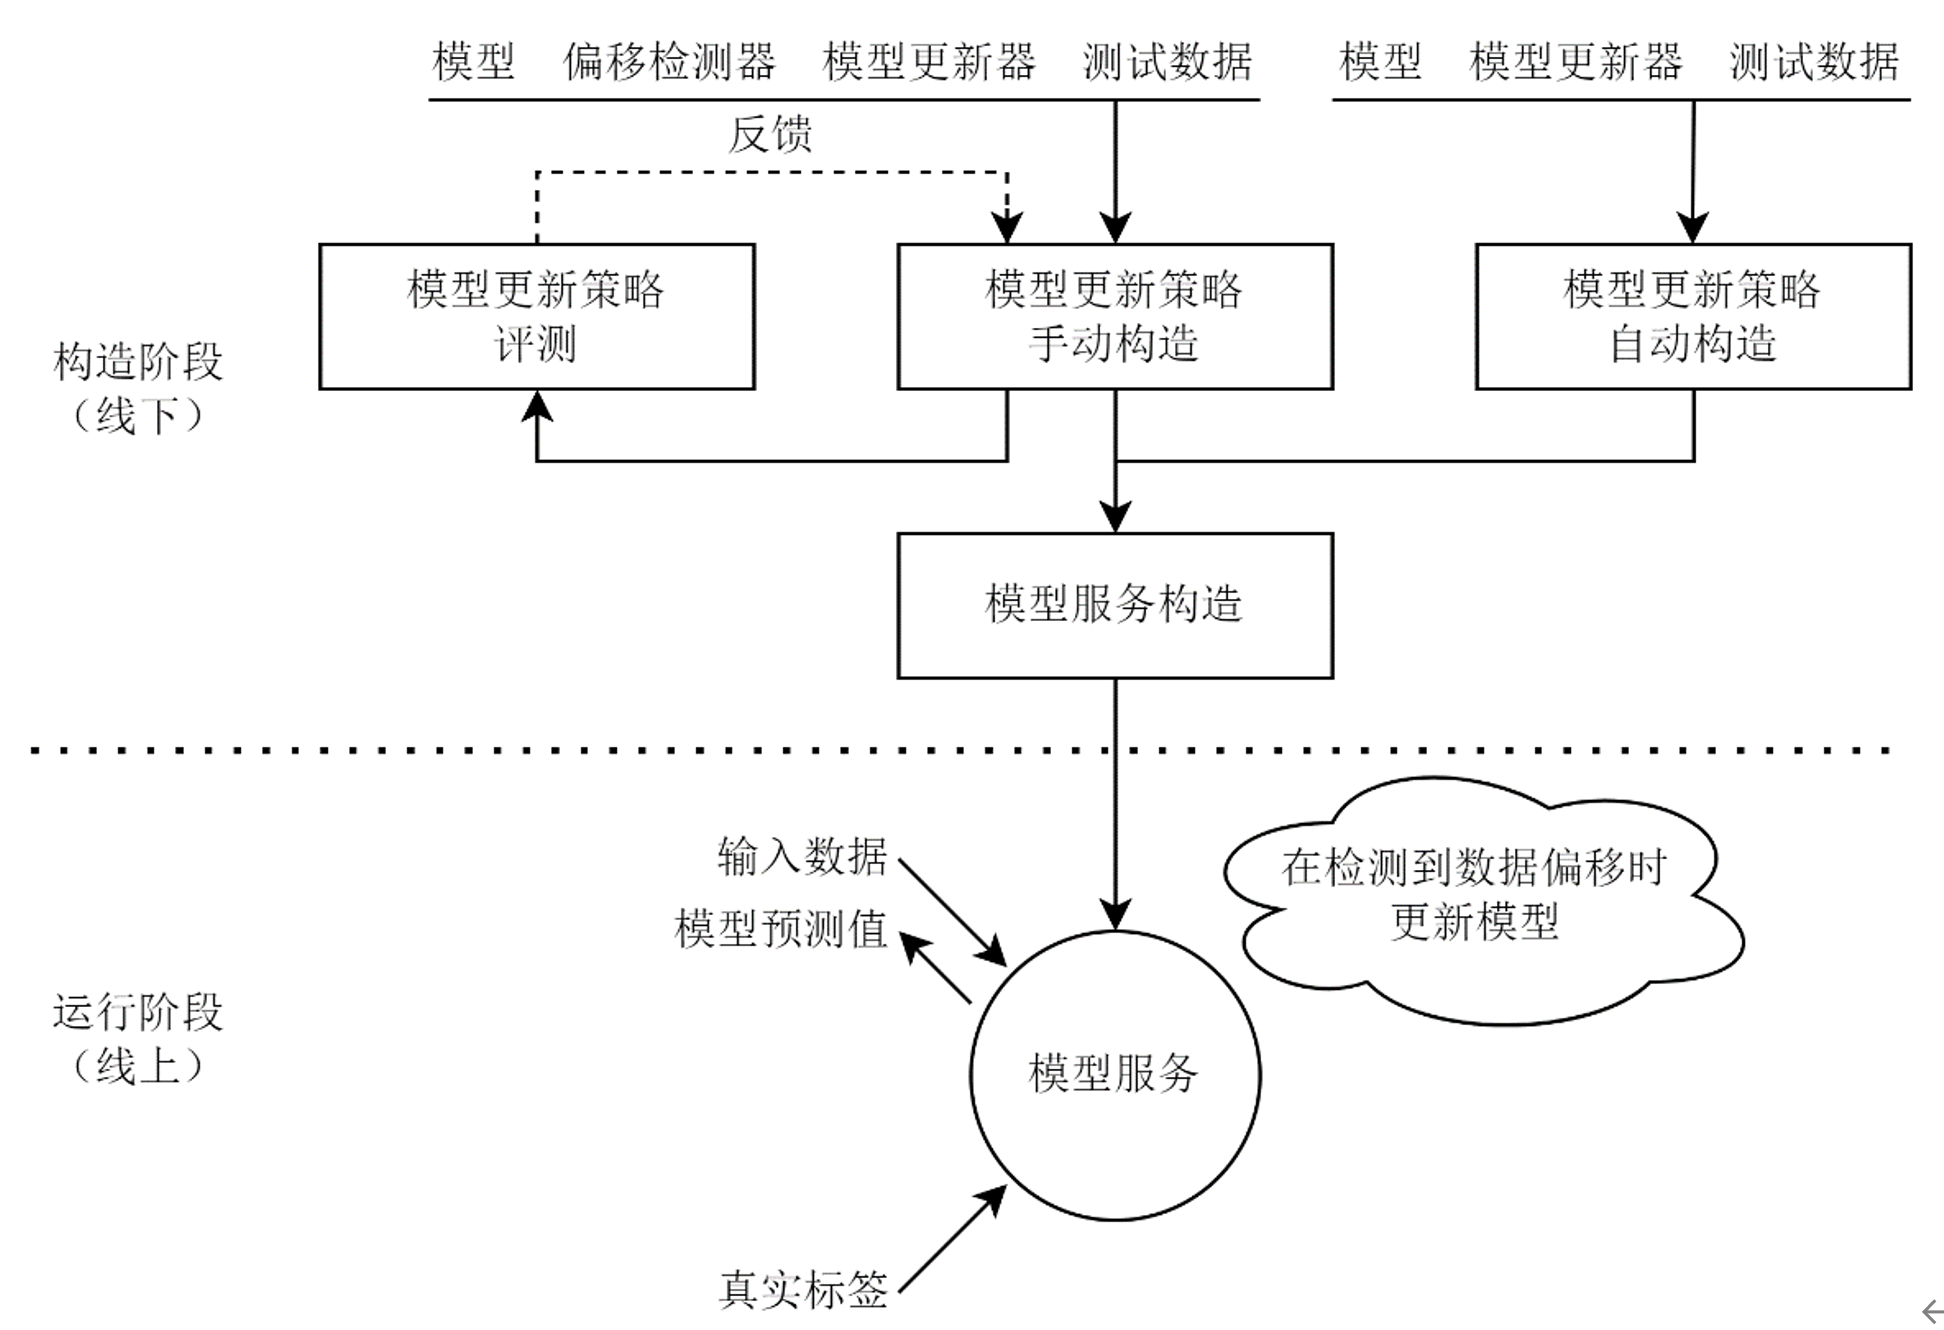
\includegraphics[width=0.8\linewidth]{model-update.png}
  \caption{模型更新策略评测与推荐流程}
  \label{fig:modelupdate}
\end{figure}

\subsection{模型服务构造}

本技术需要设计和实现一套模型服务中模型和模型更新策略的实际运行逻辑,其负责线上数据的接收和处理并成为模型服务的一部分。

在偏移检测器汇报数据偏移后,模型更新需要最近若干条样本的输入值和真实标签,模型服务内部需要一个“暂存区”来暂存已经接收到的输入值和真实标签。
考虑到基于模型效果的偏移检测器在工作时需要样本的真实标签和模型预测值来计算样本预测效果指标值,而真实标签的到来通常是有延迟的,模型服务需要把模型预测值也暂存下来。
为了让偏移检测和模型更新的过程与模型预测的过程互不干扰,除暂存区外,模型服务还需要一个独立的“偏移检测线程”来把暂存下来的数据发送给偏移检测器并在偏移检测器汇报数据偏移后执行模型更新。

\subsection{模型更新策略评测}

针对模型服务中模型和模型更新策略的实际运行逻辑,本技术需要设计和实现相应的模型更新策略评测功能。
研发人员给定模型、模型更新策略和带时间戳的测试数据,即可通过评测来模拟模型服务在实际运行时的情况并获得模型全局评价指标等与模型更新策略好坏有关的信息。

为实现符合生产环境实际情况的精确评测,本技术的评测方法将依据研发人员所给定的带时间戳的测试数据来一步步地执行模型服务偏移检测线程的步骤,同时推算其实际运行过程中每一步的完成时刻,进而在模型服务各个时刻状态的基础上推算出每个样本的预测值,最后得到模型全局平均预测效果指标。

为实现评测逻辑与模型服务实际运行逻辑的解耦,本技术还将提出一种把模型服务视为黑盒的评测方法,该方法将按照时间间隔来把各条数据发送给模型服务,同时一旦发现模型服务进入等待下一条数据的空闲状态,就立即发送下一条数据。
为检测模型服务的空闲状态,该评测方法将要求模型服务维护一个“活跃计数”,该计数的大致含义是“当前相关活跃线程的数量上界”。
这样一来,只须检测活跃计数下降到零的事件,就能检测模型服务的饥饿状态。

\subsection{模型更新策略自动构造}

在模型更新策略评测功能的基础上,本技术需要设计和实现模型更新策略的自动构造功能。
研发人员给定模型、模型更新器和带时间戳的测试数据,即可由该功能自动选择合适的偏移检测算法和参数取值(还可以包括模型更新器的参数取值,如微调学习率和迭代次数),进而形成构造模型服务所需的模型更新策略。

模型更新策略自动构造本质上是对偏移检测器和模型更新器的超参数优化。
考虑到影响模型更新策略优劣的因素不但包括模型预测效果指标还包括模型更新的计算成本代价,本技术需要实现模型更新策略的多目标优化;
针对偏移检测器的超参数优化,为降低研发人员的使用门槛,本技术需要定义一套合理的默认搜索空间以达到无须研发人员手动指定的效果;
为充分利用计算资源,本技术需要设计和实现一套易于研发人员使用的多CPU核心和多GPU并行搜索机制。

\begin{figure}
  \centering
  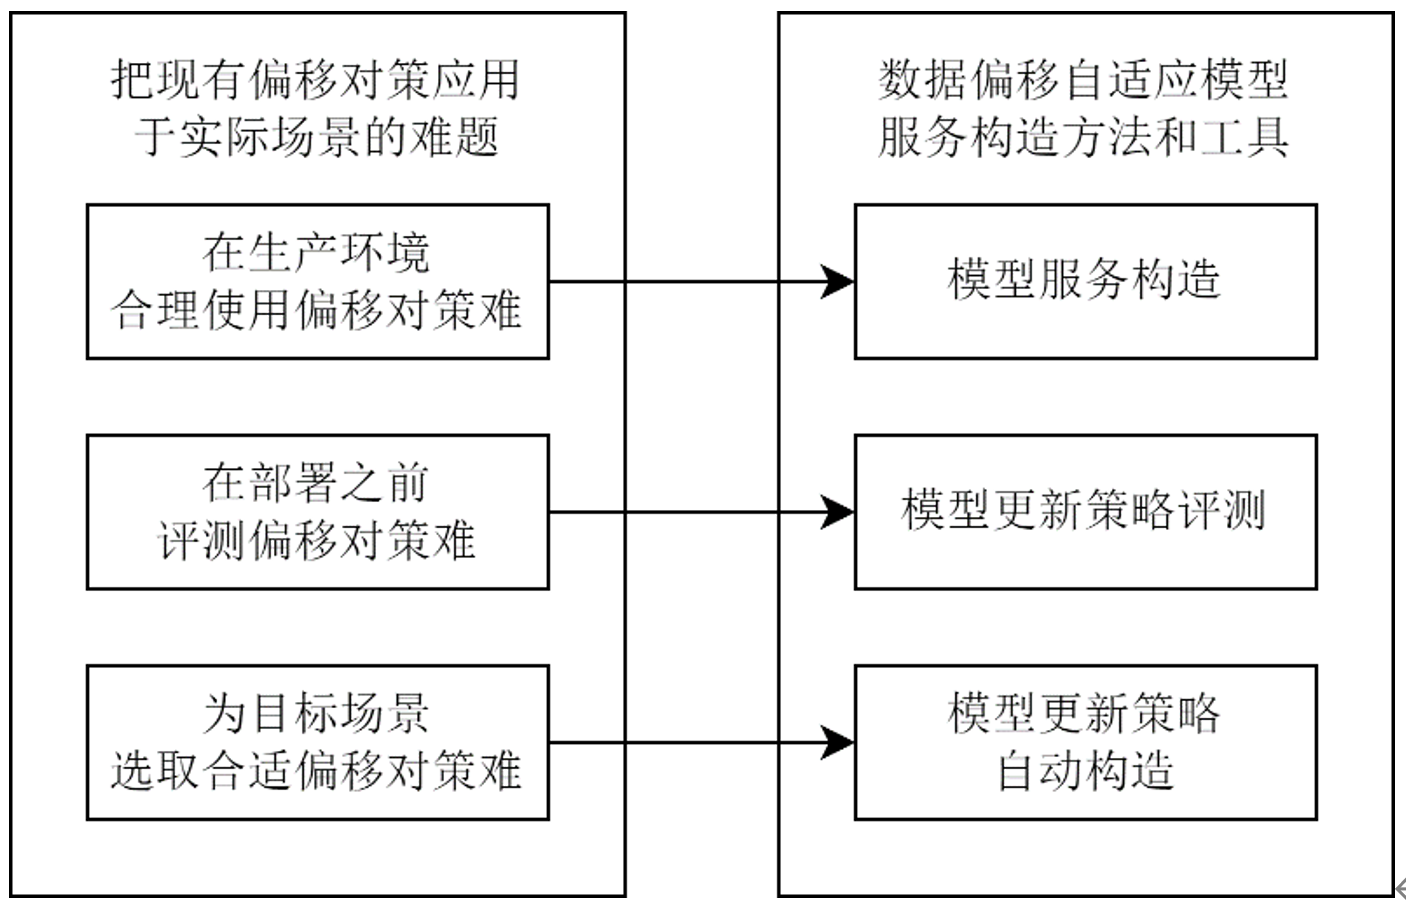
\includegraphics[width=0.5\linewidth]{model-update-auto.png}
  \caption{模型更新策略自动构造}
  \label{fig:automodelupdate}
\end{figure}
